\documentclass[12pt,a4paper,twoside,openright]{book}
\usepackage[latin1]{inputenc}
\usepackage{amsmath}
\usepackage{amsfonts}
\usepackage{amssymb}
\usepackage{latexsym}

\usepackage{graphicx}
\usepackage{multirow}
\usepackage{stfloats}
\usepackage{setspace}

\usepackage{amsfonts,psfrag,fancyhdr,layout,appendix,subfigure,url}
\usepackage[sectionbib]{natbib}
\usepackage{chapterbib}
\usepackage{makeidx}

\usepackage{listings}
\usepackage[usenames]{color}

\usepackage{layout}

\lstnewenvironment{htmlCode}[1][]
{\lstset{basicstyle=\small\ttfamily, columns=fullflexible,
keywordstyle=\color{red}\bfseries, commentstyle=\color{blue},
language=html, basicstyle=\small,
numbers=left, numberstyle=\tiny,
stepnumber=1, numbersep=5pt, frame=shadowbox, #1}}{}

\lstnewenvironment{sqlCode}[1][]
{\lstset{basicstyle=\small\ttfamily, columns=fullflexible,
keywordstyle=\color{red}\bfseries, commentstyle=\color{blue},
language=SQL, basicstyle=\small,
numbers=left, numberstyle=\tiny,
stepnumber=1, numbersep=5pt, frame=shadowbox, #1}}{}

\lstnewenvironment{pythonCode}[1][]
{\lstset{basicstyle=\small\ttfamily, columns=fullflexible,
keywordstyle=\color{red}\bfseries, commentstyle=\color{blue},
language=C++, basicstyle=\small,
numbers=left, numberstyle=\tiny,
stepnumber=1, numbersep=5pt, frame=shadowbox, #1}}{}

\usepackage{algorithmic}
\usepackage{algorithm}
\usepackage[english]{babel}
\usepackage{phdthesis}
\usepackage{longtable}
\usepackage{textcomp}
%\usepackage[T1]{fontenc}

\renewcommand{\algorithmicrequire}{ {\bf Input: } }
\renewcommand{\algorithmicensure}{ {\bf Output: } }
\renewcommand{\algorithmiccomment}[1]{/*\textit{#1}*/}
\newcommand{\HRule}{\rule{\linewidth}{0.5mm}}

\hyphenation{xe-no-pa-tient}

\newcommand{\Xeno}{Xeno Management Module}
\newcommand{\Tissue}{BioBank}


% Set equal margins on book style
%\setlength{\oddsidemargin}{40pt}
%\setlength{\evensidemargin}{40pt}
\setlength{\marginparwidth}{0pt}
\setlength{\footskip}{30pt}
\setlength{\headheight}{15pt}

\title{LAS: Laboratory Assistant System}
\author{Piero Alberto}

\makeindex
\begin{document}
%\layout
\frontmatter

\begin{titlepage}

\begin{center}

% Upper part of the page
%\epsfig{file=./logo.eps, width=0.15\textwidth}

\textsc{\LARGE POLITECNICO DI TORINO}\\[1cm]

{ \huge \bfseries Xeno Management System: User Manual}\\[1cm]

\includegraphics[width=0.25\textwidth]{./logo.eps}\\[1.5cm] 


\vfill

\end{center}

\end{titlepage}
\thispagestyle{empty} 

\mbox{}
\newpage

% Remove parskip for toc
\setlength{\parskip}{0ex plus 0.5ex minus 0.2ex}

\setcounter{page}{1}
%\onehalfspacing %interlinea
%\doublespacing
%\pagestyle{fancy}
%\fancyhead[RO]{\emph{Contents}}
%\fancyhead[LE]{\emph{Contents}}

\tableofcontents
\listoffigures
\listoftables
% Dutch style of paragraph formatting, i.e. no indents.
\setlength{\parskip}{1.3ex plus 0.2ex minus 0.2ex}

\mainmatter

\chapter{Introduction}\label{chap:intro}

The cancer is a disease whose cure is still a subject of several research projects. The cancer has developed several therapies such as chemotherapy and radiotherapy. A new branch of studies aims to develop targeted drugs capable of affect only damaged cells without harming healthy ones still inside the body. This approach involves the production of large amounts of data, making essential the presence of an efficient information management.

Many efforts have been devoted to the development of data management systems related to cancer research. One of the main ICT technologies used in research laboratories is the Laboratory Information Management Systems (LIMS). Many commercial LIMS are available, but are usually very expensive and require a large amount of human and economic resources to fit the specific requirements of each laboratory. However, also exist a number of LIMS proposed by the research community, released as open-source projects. Certain manage data related to some specific research procedures. Other LIMS focus on the management of data associated with the mice used in research, monitoring the various colonies of animals. However, all these systems are mainly focused on the management of some types of highly specific data relating to a particular series of experiments.

To overcome the main problems of the approaches mentioned above and to satisfy the requirements deriving from the activities of research laboratories, the research team DBDMG the Polytechnic of Turin, in collaboration with the staff of IRCC of Candiolo, proposes the Laboratory Assistant Suite (LAS), a platform which assists researchers in the various laboratory activities. Its modular architecture makes it possible to manage different types of raw data (for example, organic molecules), and tracking of experimental data. In addition, the platform supports the integration of different resources when performing a series of tests in order to extract information about the analyzed tumors. The user interfaces are designed to help manage the data in harsh environments, where researchers need to minimize their interactions with the system (for example, under sterile conditions).

At IRCC of Candiolo, researchers perform studies and research on so-called xenopatients. These are immunosuppressed mice in which are inserted fragments of cancer tissue from human subjects, to be able to study the reactions to certain drugs. In this way, the aim is to obtain a specialized drug treatment for each type of tumor under study. Within the LAS \Xeno\ (XMM) is the operational level. is a module that can send information requests to the modules above. Its task is to manage data and experiments on xenopatients. 

XMM aims to track and monitor all activities related to xenopatients and their life cycle, starting from the moment they are delivered from suppliers at the institute. It should then be able to handle these operations, implementing features and interfaces in ways that meet the specific demands by IRCC of Candiolo. An example is the requirement of compatibility with devices for reading barcodes and RFID microchip. In addition, it must be usable by mobile users, such as tablets.

The developed system, named \Xeno\ (XMM), allows you to track and monitor all activities related to research and study xenopatients and their life cycle. The user interfaces are designed to help manage the data in harsh environments, where researchers need to minimize their interactions with the system. XMM offers a work environment capable of simulating the laboratory, where researchers work every day. This allows for reducing the errors during data entry, especially in dedicated interfaces to the operations of implants and explants.

The life cycle begins with the loading of new xenopazienti in the system. The interface developed for this feature allows a quick integration of new mice, especially if you are using the RFID reader. The cycle continues with implants, surgical procedures through which you insert a piece of tumor tissue in the body of the mouse. At this stage, you select a xenopatient and an aliquot.

An implanted mouse may be subject to measurement, with the aim of controlling the tumor growth. The managed measurements are divided in two types: qualitative and quantitative. The first is a subjective measurement, determined by the operator's discretion and obtained by palpation of xenopatient. The second is obtained electronically through a special electronic caliber, which can return the dimensions of the tumor being studied. The system minimizes the interactions between the user and the system, interfacing directly with the tools of reading. A mouse, after the measurement, can be associated with a planned treatment or for explant. The treatments allow you to test determined drugs on xenopatients, to try to determine their effectiveness. Each treatment consists of several steps, each of which corresponds to a given dose of medication. If the operator wishes to associate a set of xenopazienti to a treatment that does not exist yet, it can be defined through an interface, where a Gantt chart allows you to schedule the various steps.

The last phase of this cycle of life is represented by the explants, with the surgical procedure which removes the tumor from xenopatient, implying a sacrifice. From the removed material are created multiple fragments of tissue, which will be available for new implants on other mice. The interface implemented for simulating the real environment explants laboratory, offering a software work simple for the operator. The system provides the user the ability to interact with the screen quickly.

\chapter{Application context}\label{chap:xenocontest}

\section{Introduction}

In pathology, a tumor is an abnormal mass of tissue that grows in excess and in an uncoordinated mode with respect to normal tissues, and persists in this state after the termination of the stimuli that have led the process, making it hereditary damage, against new cells.

For a cell becomes cancerous, it must accumulate a series of damages to its system of control of reproduction. In fact, cancer is a genetic disease of somatic cells. Every cancerous cells show alterations, often very large,of their chromosome structure: the number of chromosomes in the nucleus can be altered and their chromosomes are damaged, missing or multiple. Cancer can affect all tissues, especially those subject to various stress and subject to continuous exchange, as, for example, skin, respiratory tract and intestine.

The colorectal cancer (\textit{CCR}) is widespread, with high mortality in Western countries. Is the second leading cause of death among cancer patients, both in man and woman. The incidence shows considerable variation according to different geographical areas. In the U.S. it settles on 45-50 cases per 100,000 population per year, in the UK is around 25-30 cases, while in Japan does not exceed 10-12 cases per 100,000 inhabitants per year. Italy is among the countries with intermediate incidence rate, with about 35 cases per 100,000 population per year and presents significant differences from region to region. The CCR is rare under the age of 50, and its incidence increases rapidly with age, doubling every decade between 40 and 70 years. The average age at diagnosis is about 69 years old for men and 72 years old for women.

The IRCC is an institute of Candiolo responsible for research and treatment of cancer. At the institute, are conducted several experimental protocols, with the use of laboratory experimental mice in order to identify and develop new treatments for cancer. Research studies currently are focusing on colorectal cancer (CCR).

\section{Approaches to cancer - Target Therapy}

The main problem in cancer therapy is that, in general, being a cancer composed of cell essentially very similar (if not for some genetic damage) to the rest of the body, drugs active against cancer cells are usually also very toxic to normal cells. For this reason, a fundamental objective in oncology research is by the action \textit{targeted drugs}, resulting in a therapeutic window. Any drug developed for act against cancer cells must be tested carefully to make sure also that will not damage healthy cells in the body.

The high rate of replication of cancerous cells makes them more vulnerable to radiation than normal tissue. This weakness is exploited to heal many types of solid tumor with radiation (\textit{radiotherapy}, bombardment with gamma rays) in an effort to kill as many cancer cells as possible. On other hand, the \textit{chemiotherapy} exploits the sensitivity of individual tumors to specific substances. Since the sensitivity of the tumor depends also on the patient's immune system is usually designed a custom blend of several drugs for each patient. Almost always, this cocktail contains one or more inhibitors of mitosis, such as taxol and its derivatives to prevent cellular proliferation. Some of these inhibitors are primarily responsible for alopecia (hair loss ) that afflicts patients undergoing chemiotherapy.

The cancer develops and progresses as a result of a genetic lesion, that is an alteration of the DNA in an adult cell. So turn off the genetic lesion that produced the means compromising tumor its growth. The targeted therapies, developed over the past 20 years, are indeed able to block the function of genetically altered molecules in the tumor without affecting normal tissues and therefore without causing a general body damage.

These therapies are useful only in subjects with a tumor that contains, in the DNA, the anomaly which makes the tumor susceptible to the drug targeted. This approach also has diagnostic and therapeutic challenges, necessarily, the traditional classification of neoplastic diseases.

In the context of cancer therapy targets are no longer defined by place of occurrence and morphological characteristics, but also on the basis of the molecular lesion that characterizes them and , at the same time, makes them vulnerable to a particular treatment. New therapies are therefore not only targeted, but also personalized. The molecular diagnosis refers to the need to precisely characterize each patient for various genetic mutations that presents the tumor and, therefore, makes it sensitive to a drug and resistant to others.

\section{Xenopatients}\label{sez:xp}

At the Institute of Candiolo it was decided to create a platform for preclinical investigations which best approximates the context of real tumors. The project involves the recovery of surgical pieces (samples) from surgery, with the informed consent of patients. The sample is stored under conditions that ensure the vitality and then is implanted in a receiving animal, usually under the skin of an experimental mouse. The animal becomes a "small patient" that is subjected to experimental therapies. For this, we define the mouse that brings with it the human cancer \textbf{xenopatient}. The choice fell on mice because they have a DNA structure very similar to that of humans. In addition, allow for a wide range of organisms on which to make tests at a reduced cost. Finally, these mice are delivered already immunosuppressed, with the immune system very weak, so they are more susceptible to other infections, because their weakest.

The experimental animals are farmed directly in the institution (to make economically sustainable the research), through the maintenance of a breeding colony (\textbf{breeding}) that generates the animals on which experiments are actually carried out (\textbf{experimental}).

The study enables the execution of \textbf{large-scale genetic analysis} of the tumor, in order to identify lesions that potentially are susceptible to attack with the experimental drugs. In the presence of a lesion, the xenopatient is treated with the drug target and response to treatment is monitored. In case of positive result the next step is to transfer the information to the clinic and begin to treat real patients (but only those with the genetic defect that responds to therapy) with the drug that has shown efficacy in xenopatients. In other words, the preclinical xenopatients allow the personalization of targeted therapies.

Among the available drugs for the treatment of colorectal cancer, cancer of the head and neck and, according to recent studies, also lung cancer, is administered the \textbf{Cetuximab}, a monoclonal drug, produced in a mammalian cell line by recombinant DNA techniques. Even the IRCC of Candiolo used this drug, testing it on patients and on xenopatients.

Efficacy evidence of the Cetuximab as a treatment of colorectal cancer are numerous. With the administration of this drug, alone or in combination with traditional chemotherapy drugs, in patients refractory to classical treatments (chemotherapy alone), is achieved an increase in response rate, disease control, disease-free survival.

Even when used in first line (early in the disease), has been shown to increase the positive effects of the chemotherapy also to allowing more patients to achieve a reduction in tumor size. Unfortunately, not all the population that the drug is administered benefits from the positive effects of Cetuximab. For this reason a number of years of scientific research is investigating the possible existence of factors that can predict response to therapy. Although some markers have been identified predictors, to date there is no marker that can identify with sufficient sensitivity and specificity patients who respond adequately to treatment with Cetuximab. The identification of these markers would be extremely useful to apply the medication in a selected population is under the first line and second-line allowing you to reduce costs, avoid non-responding patients to unnecessary treatment burdened by adverse effects and improve the selection of personalized therapies

The key point in order to conduct the study is to obtain a good engraftment of the tumor samples in mice. As can be imagined, if the tumor will not grow in the tissues of xenopatients, can not do experiments. The goals of these operations are basically two. The first consists in the expansion of tumor material, with the purpose of collection material. The second, however, meets the objective of having to perform experimental treatments.
In the figure~\ref{fig:schema} is shows the general pattern of the flow of operations on xenopatients, placed in the context of the institution. 
%Below are detailed steps in the image.
\begin{figure}[h]
\begin{center}
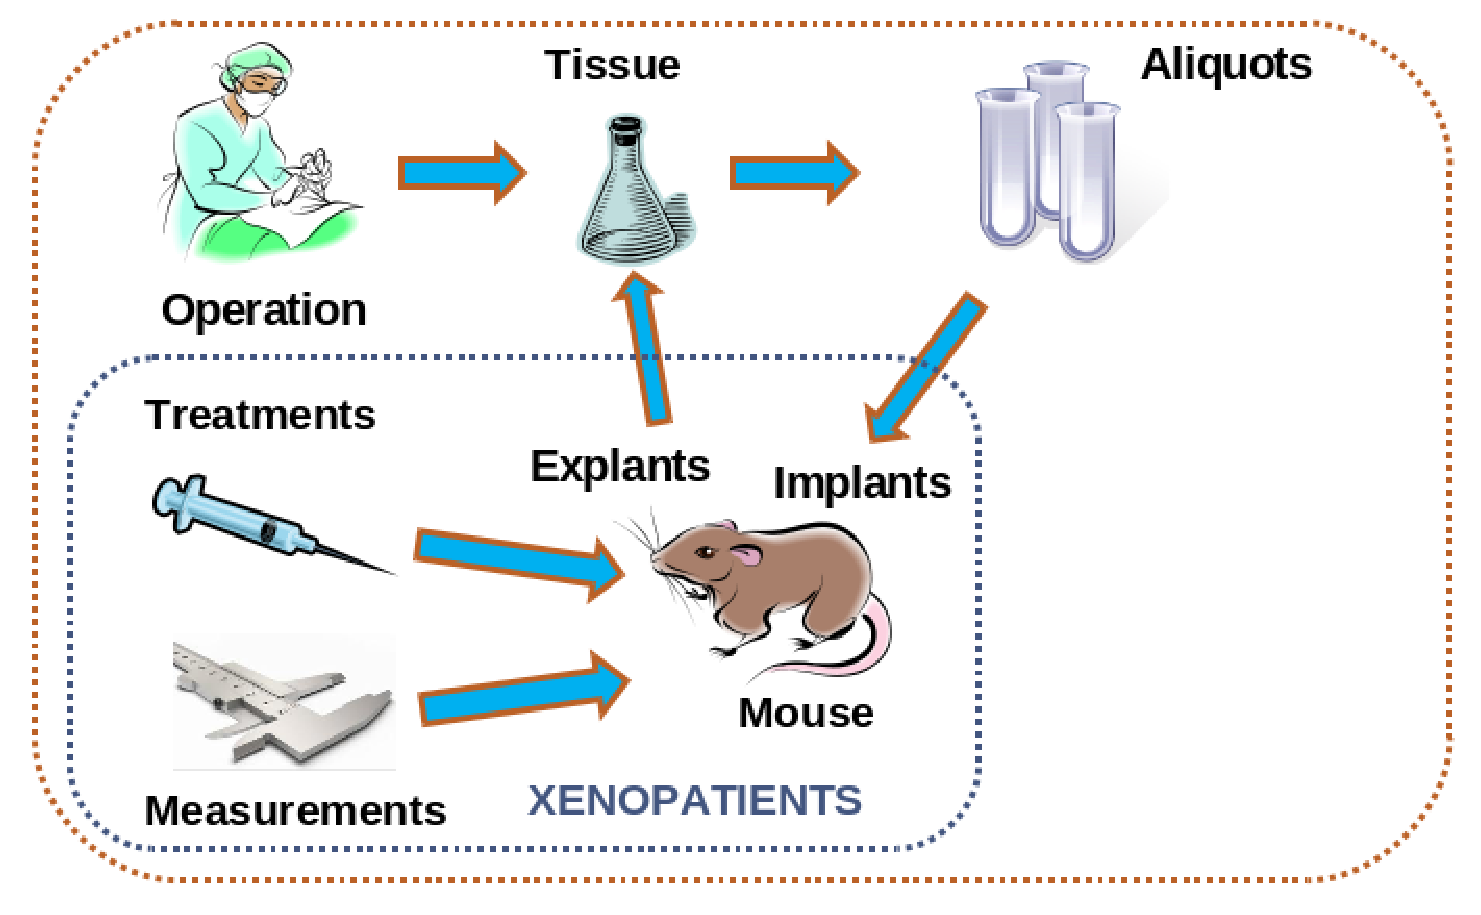
\includegraphics[width=0.8\textwidth]{./Figure/schema}
\end{center}
\caption{Operational flow on the xenopatients}\label{fig:schema}
\end{figure}

The procedure adopted involves various stages. The first takes place in the surgery room where surgery is the sample collected fresh.

Later, in conditions close to the maximum sterility, it's taken a part of the sample of tumor, and then divide the portion into several fragments. Each fragment is stored inside the tubes. Thereafter, the samples are brought to the operating table veterinarian for \textit{implant} in mice. The aims of the plants may be testing some drugs or the production of tumor tissue, using mice as an incubator.

To evaluate the efficacy of \textit{treatment} with the targeted drug, it is necessary to derive from a single tumor xenopatients a court sufficiently large to be divided into two groups, one of the treaties and that of the untreated (\textit{control group}).

A treatment is the administration of one or more drugs to xenopatients, with a precise scheduling and length of time. We also distinguish \textit{acute treatments}, which require mandatory explant of mice on which they are performed, ​​in order to identify and study the behavior of biomarkers in drug response.

Controls are carried out on tumor growth by palpation of the lesion in the plant or by measuring with a caliber. With these measurements it is possible to evaluate the effectiveness of a treatment . In fact, If there is a slowdown or a halt in tumor growth, it appears that the treatment is achieving the goal.

Then, there comes the sacrifice of the mice through a lethal dose of anesthetic. The tumor is removed and it is divided into several fragments. It performs this procedure for each of the implanted xenopatients for which explant is requiredo.

Through the operation from explant of the tumor by xenopatients, is possible create a variety of new rates to be, for example, implanted in other mice. Doing so creates an evolution of the original tumor, passing from mouse to mouse, and keeping it alive. On this basis, we can introduce the concept of genealogy of xenopatients. They belong to the same lineage the mice that received the same plant tissue, derived from a single progenitor xenopatients. Taking advantage of the genealogy of the tumor, it is possible see its progress in the different generations, with different responses to various treatments and engraftment.

\ Xeno \ born in this context, with the aim of managing the data on of xenopatients and, in particular, all the information about the life cycle of a mouse, such as measurements and pharmacological treatments. Although current studies are focused on the CCR, the developed application is able to manage all information relating to of xenopatients regardless of the type of cancer studied.

\chapter{Casi d'uso}\label{chap:xenocase}

Questo Capitolo raccoglie tutti principali casi d'uso sviluppati per \Xeno. Con la dicitura `caso d'uso', ci si riferisce ad una tecnica usata nei processi di ingegneria del software, per effettuare in maniera esaustiva e non ambigua, la raccolta dei requisiti per produrre un software di qualit\`a e in linea con le specifiche richieste.

L'analisi dei casi d'uso verr\`a affrontata categorizzando gli argomenti della Web Application in macro funzionalit\`a. La suddivisione qui utilizzata corrisponde alle suddivisioni utilizzate per la creazione del menu di \Xeno, ovvero:
\begin{itemize}
	\item \textbf{caricamento xenopazienti} nel sistema;
	\item \textbf{aggiornamento dello status} di uno xenopaziente;
	\item \textbf{misurazioni}, divise in \textit{misurazioni qualitative} e \textit{misurazioni quantitative};
	\item gestione \textbf{impianti};
	\item gestione \textbf{espianti}.
\end{itemize}	

Nell'illustrare i vari casi d'uso, si proceder\`a illustrando i requisti delle varie aree, descrivendo l'interfaccia sviluppata e il flusso di dati che la caratterizza. Nella fase di sviluppo di queste interfacce, si \`e cercato di rimanere il pi\`u fedele possibile alle direttive iniziali, apportando il minor numero possibile di modifiche, in modo tale da soddisfare al meglio i bisogno dell'IRCC di Candiolo.

In Figura~\ref{fig:useCase} \`e riportato lo schema generale dei casi d'uso. All'interno di questo Capitolo, si analizzer\`a con maggior dettaglio ogni componente di questa figura.

\begin{figure}[h]
\begin{center}
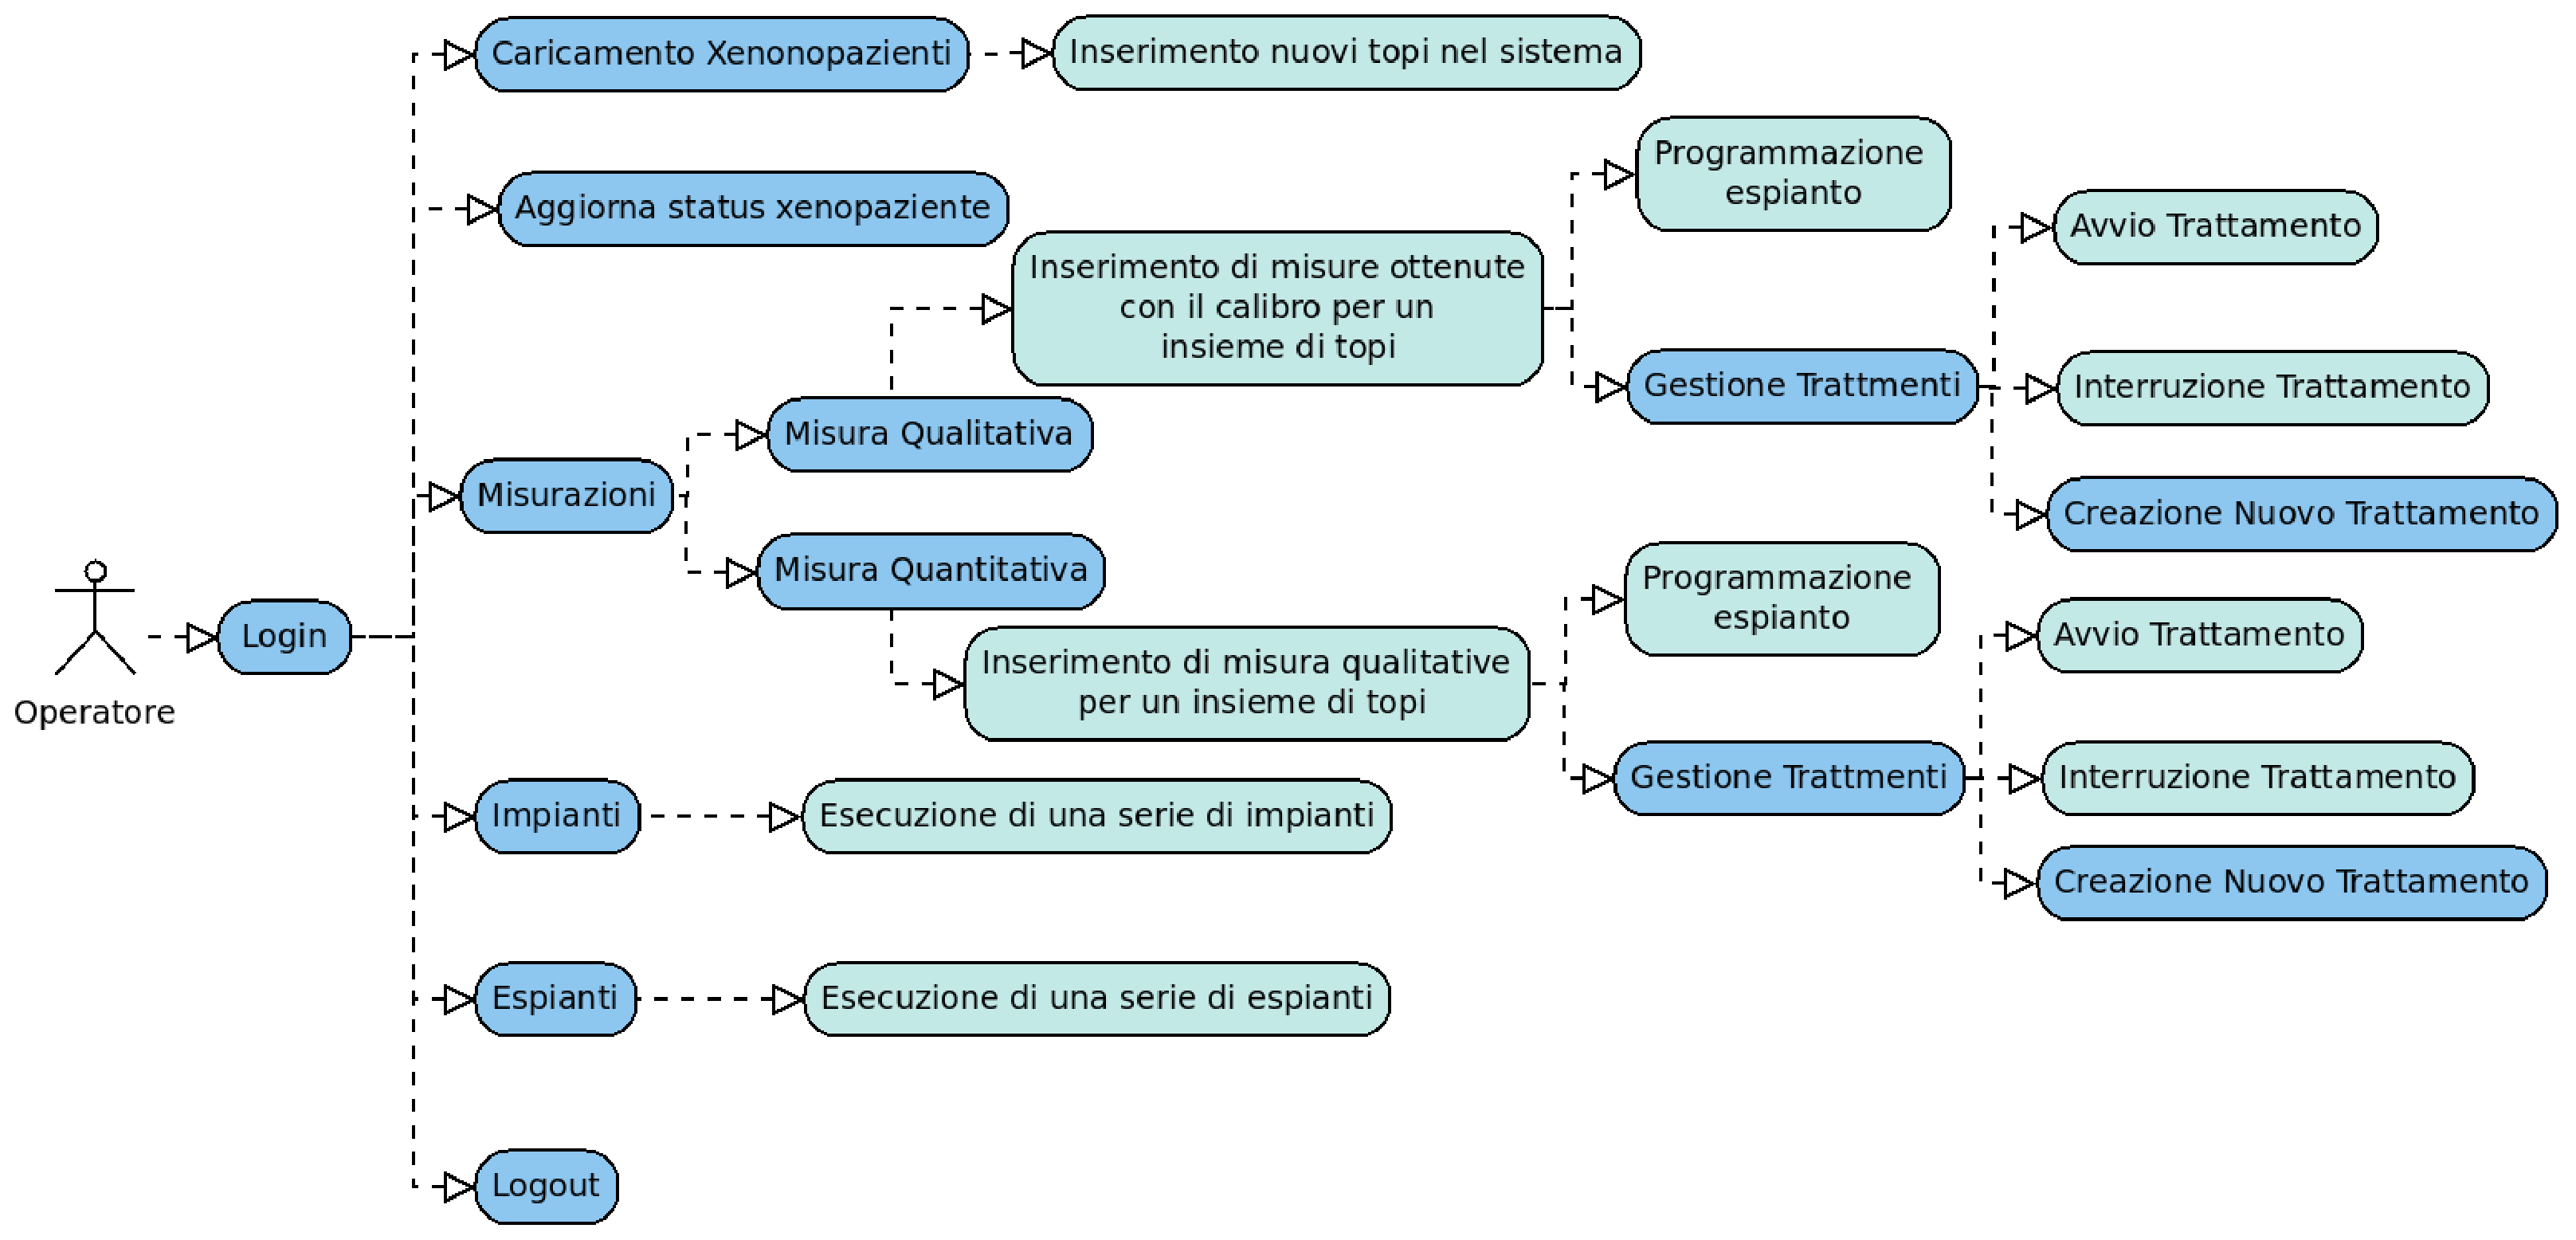
\includegraphics[width=1\textwidth]{./Figure/use_case}
\end{center}
\caption{Caso d'uso generico}\label{fig:useCase}
\end{figure}

\section{Caricamento xenopazienti nel sistema}

Questa interfaccia ha il compito di fornire all'operatore un metodo veloce ed intuitivo per immettere nel sistema i dati relativi a nuovi xenopazienti. In Figura~\ref{fig:UCDmiceL} \`e riportato il diagramma dei casi d'uso relativo a questa interfaccia.

\begin{figure}[h]
\begin{center}
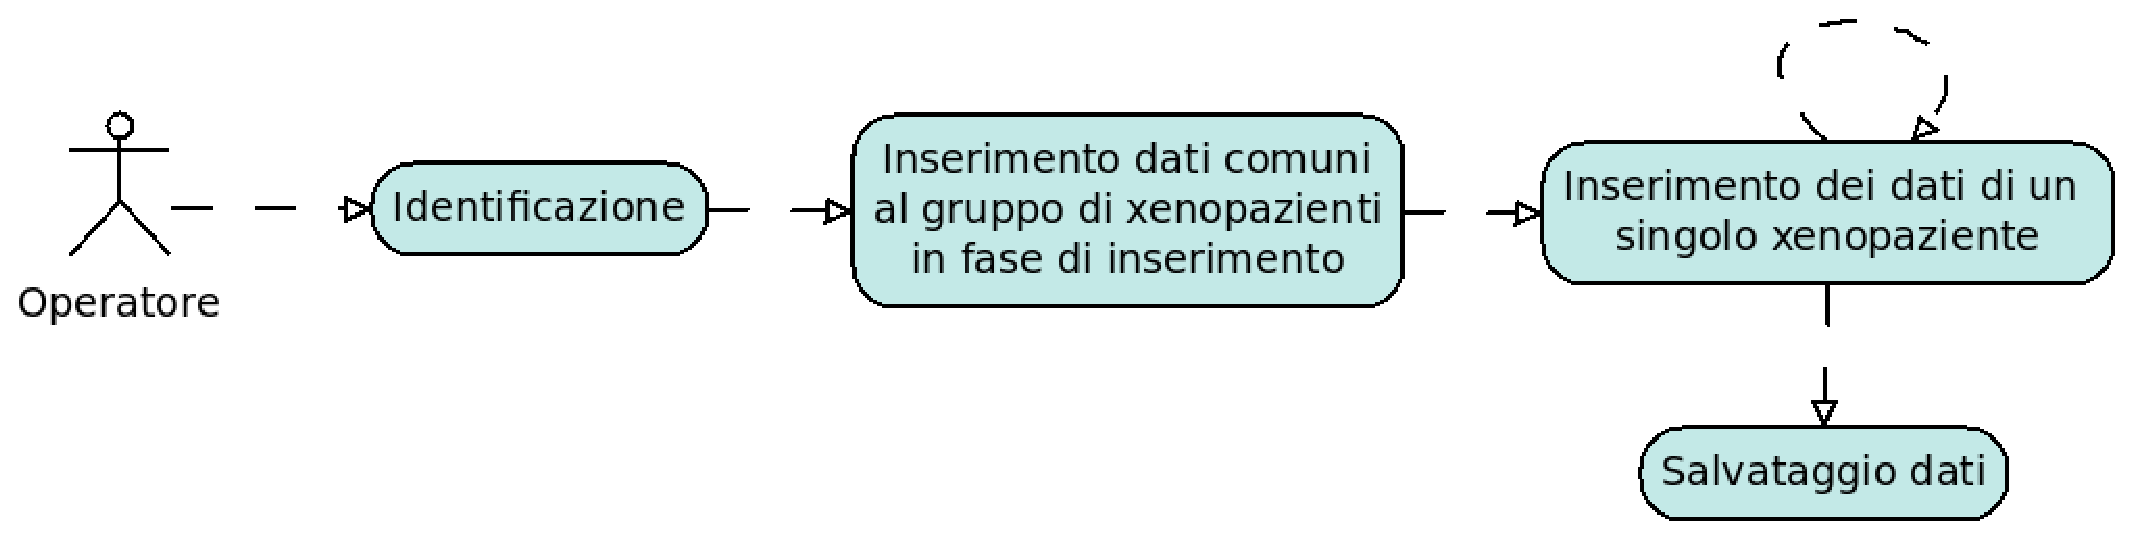
\includegraphics[width=0.7\textwidth]{./Figure/UCDmiceloading}
\end{center}
\caption{UCD del caricamento xenopazienti\label{fig:UCDmiceL}}
\end{figure}

Gli xenopazienti sono inseriti nel database in gruppi pi\`u o meno numerosi. Per snellire la procedura, all'operatore si presenta una schermata per immettere i dati comuni a tutti gli xenopazienti del gruppo. Questi dati comuni sono molteplici. Uno di questi \`e la data di disponibilit\`a, il cui valore di default \`e la data odierna, che indica la data dalla quale si possono utilizzare i topi ricevuti. Un altro parametro da inserire, molto importante, \`e lo status di partenza dei nuovi xenopazienti, selezionabile tramite un'apposita tendina. I dati proposti presenti in questa tendina sono presi dalla tabella Status del database. Inoltre, si inserisce anche l'et\`a presunta, in settimane, del carico di topi. Questa et\`a viene utilizzata per calcolare la data di nascita dei vari xenopazienti inseriti. Si inserisco anche il fornitore del carico di topi e il gruppo di ricerca al quale vengono assegnati.

Successivamente, si accede ad un'altra schermata, dove \`e possibile inserire i dati di ogni singolo topo. I dati necessari per ogni xenopaziente sono il suo barcode e il sesso di appartenenza. Si \`e quindi sviluppato un campo di testo per il barcode e due radio button, uno per i topi maschi e uno per i topi femmina. Il barcode pu\`o essere immesso da tastiera oppure attraverso l'utilizzo di un apposito lettore di microchip, leggendo il barcode in esso contenuto. \`E presente anche un tasto per confermare l'inserimento di un singolo xenopaziente, dopo averne inserito i dati. Effettuata l'immissione dellle informazioni relative ad un topo, queste vengono inserite in una lista, che mostra tutti gli xenopazienti inseriti fino a quel momento. Per velocizzare l'inserimento ed evitare di dover cliccare il bottone di conferma ad ogni topo, si \`e associato l'inserimento nella lista alla ricezione del carattere \textit{return} (invio). Questo particolare \`e molto importante per massimizzare i vantaggi derivanti dall'utilizzo del lettore di microchip. Infatti, si pu\`o associare il carattere return alla fine di ogni lettura di barcode, automatizzando cos\`i l'inserimento di uno xenopaziente con una singola operazione. In questo modo si conferisce maggior libert\`a all'operatore, il quale pu\`o effettuare le operazioni di immissione dati con maggiore velocit\`a.

Se si cercano di sottomettere dei dati errati (ad esempio una stringa in un campo riservato a numeri interi) o formatatti in modo scoretto (ad esempio, una data scritta non correttamente), i campi che li contengono vengono evidenziati da un messaggio che descrive il tipo di errore riscontrato, aiutando l'utente ad inserire i dati in maniera corretta.

Per rimediare ad eventuali errori nell'immissione dati (ad esempio, si inserisce il sesso sbagliato), si pu\`o utilizzare la funzione di cancellazione all'interna del la lista degli xenopazienti gi\`a inseriti. Questa lista ha infatti sia una funzione di riepilogo dinamico, sia la possibilit\`a di cancellare, uno ad uno, gli inserimenti gi\`a effettuati, prima dell'effettivo salvataggio nel database.

Una volta terminato, si inviano i dati al server, il quale li elabora e fornisce un report dei dati salvati, a meno che non si sia verificato un errore del sistema. In Figura~\ref{fig:SDmiceL} \`e riportato il diagramma delle sequenze di questa interfaccia, che riepiloga i vari passi descritti in precedenza.

\begin{figure}[h]
\begin{center}
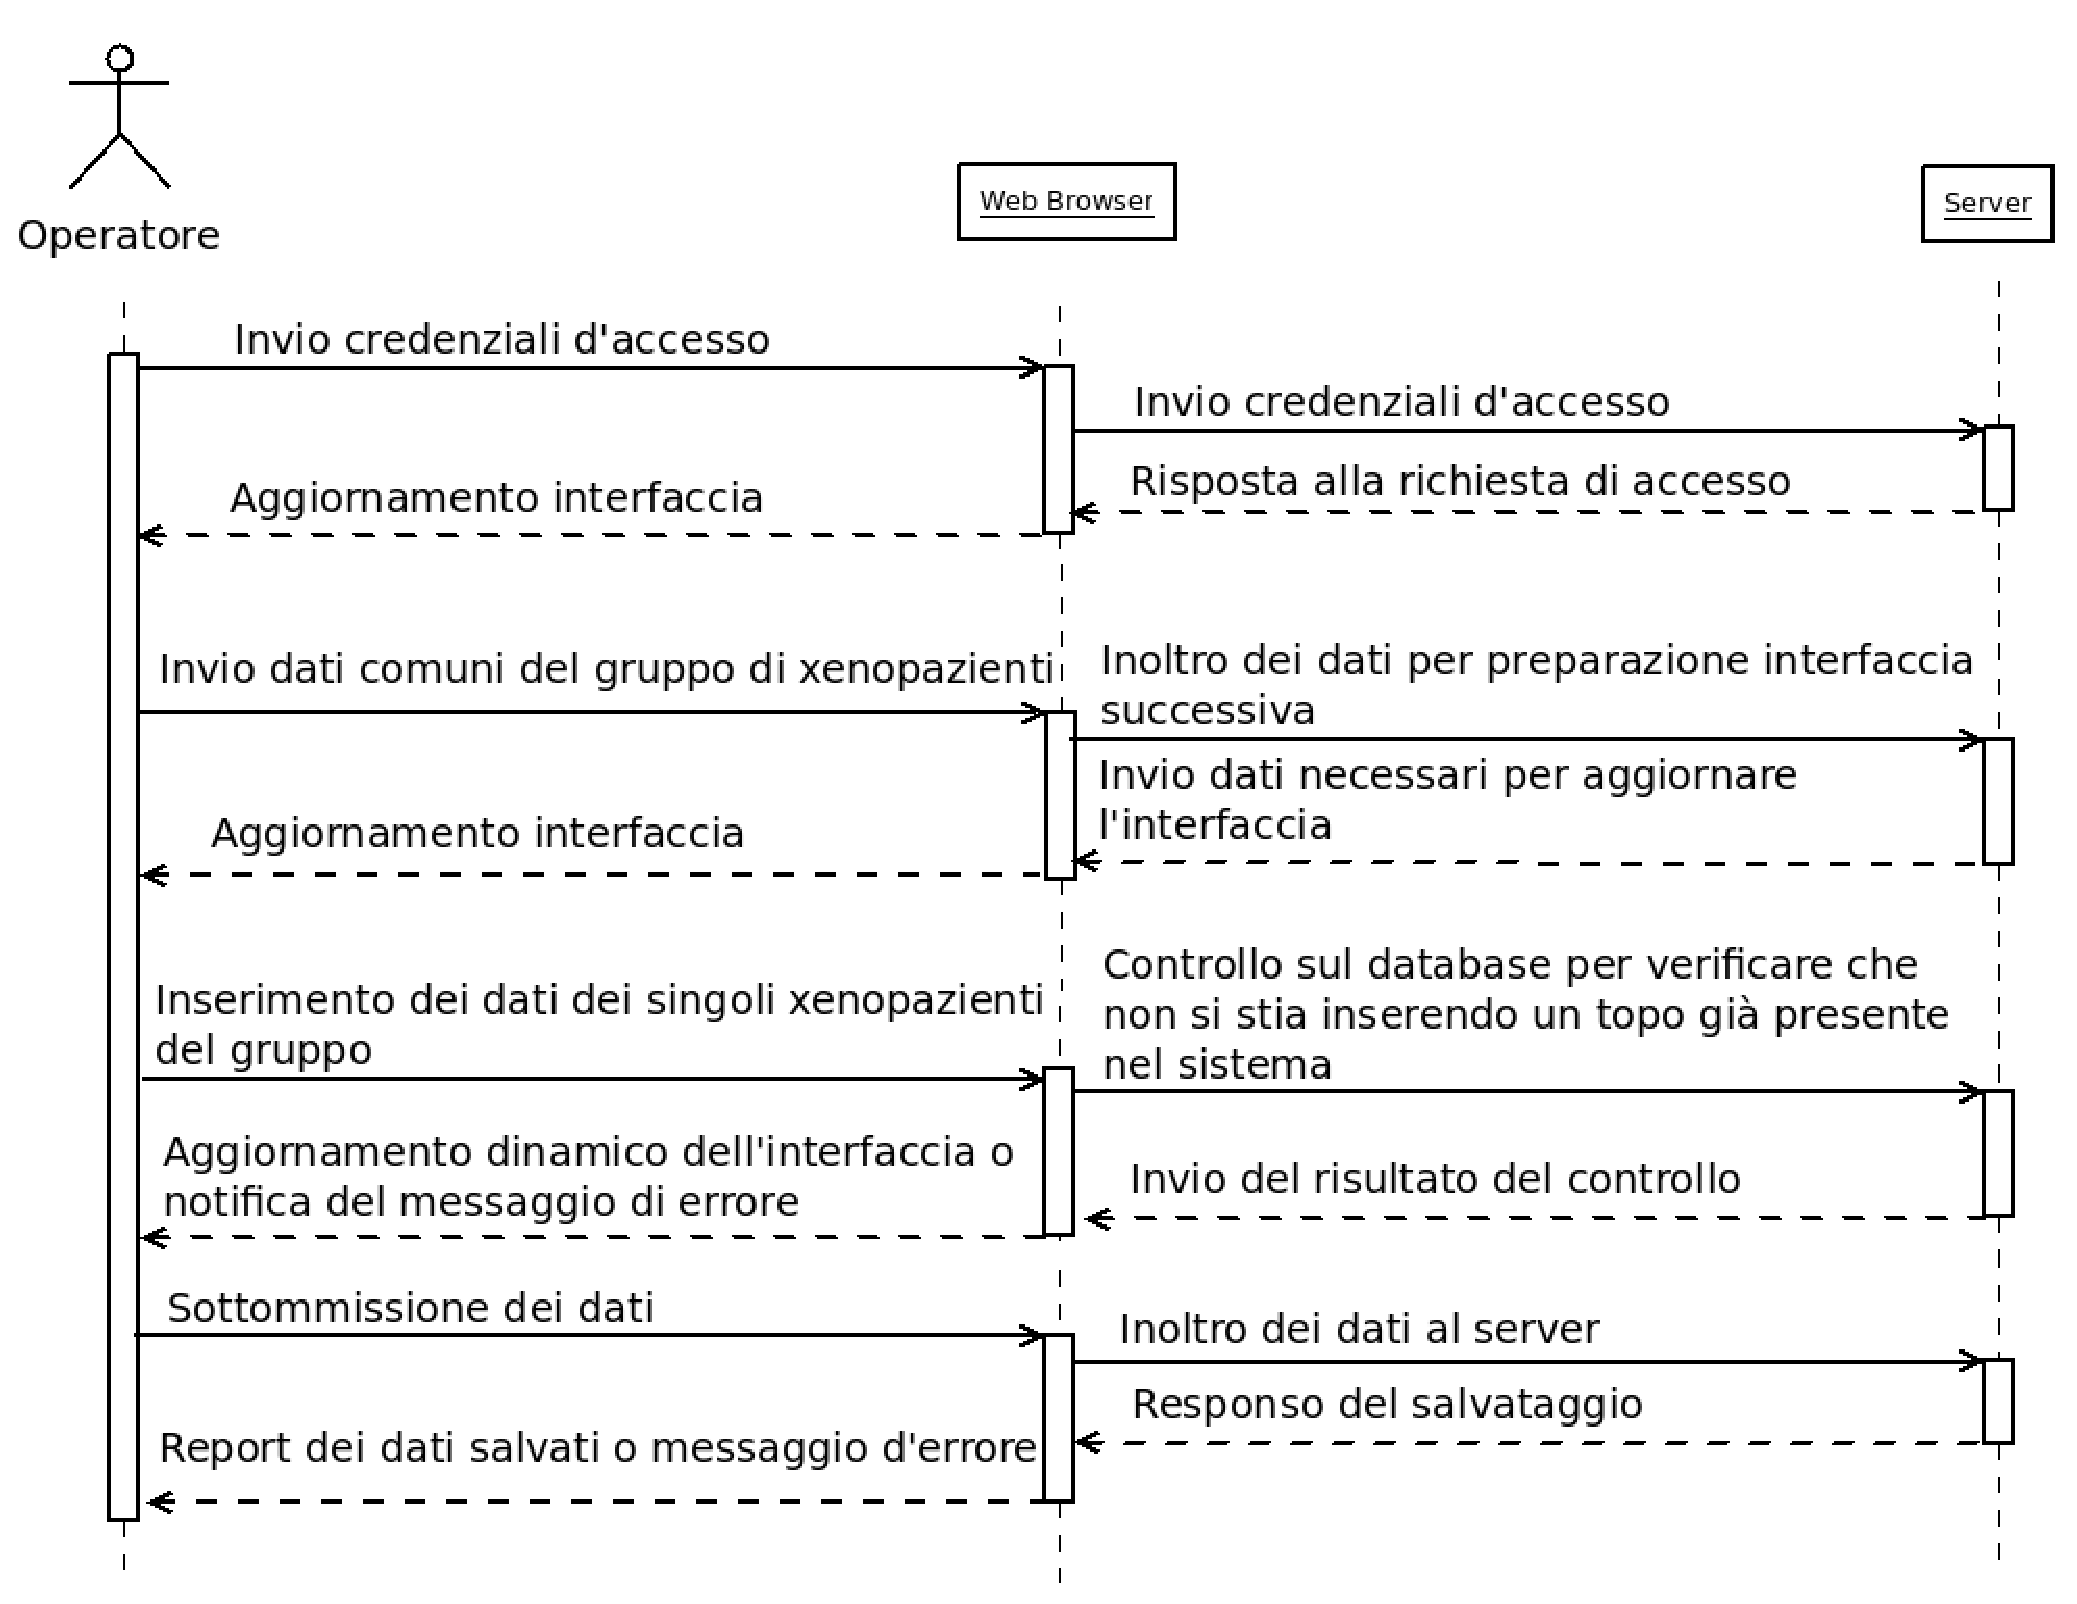
\includegraphics[width=0.7\textwidth]{./Figure/SDmiceloading}
\end{center}
\caption{Diagramma delle sequenze del caricamento xenopazienti\label{fig:SDmiceL}}
\end{figure}

\newpage

\section{Aggiornamento status degli xenopazienti}

Questa funzionalit\`a permette di cambiare lo status attuale ad uno o pi\`u xenopazienti, in modo tale da registrare il verificarsi di determinate situazioni, come ad esempio il trasferimento del topo o la morte non programmata. In Figura~\ref{fig:UCDmiceL} \`e riportato il diagramma dei casi d'uso relativo a questa interfaccia.

\begin{figure}[h]
\begin{center}
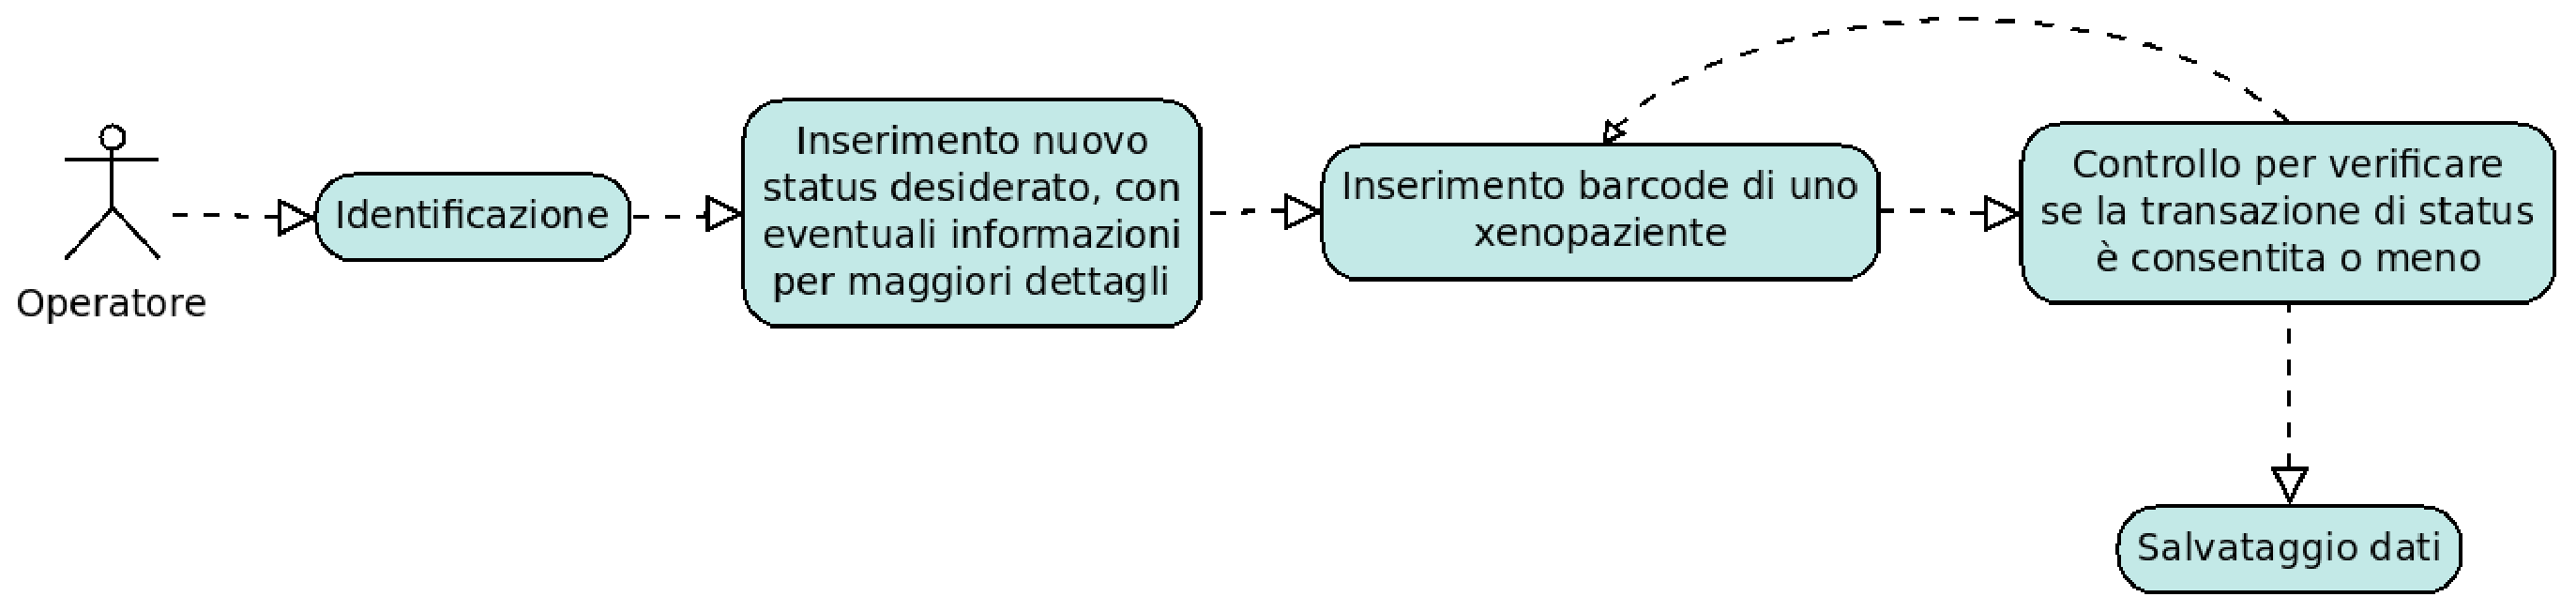
\includegraphics[width=0.8\textwidth]{./Figure/UCDchangestatus}
\end{center}
\caption{UCD dell'aggiornamento dello status degli xenopazienti\label{fig:UCDcs}}
\end{figure}

All'utente \`e inizialmente richiesto di immettere lo status da assegnare ad un gruppo di topi, inserito successivamente. Questa schermata gestisce i cambi si status non-ordinari, prelevando gli status proposti all'operatore dalla tabella Change\_status.
A seconda del nuovo status selezionato, verranno richieste o meno delle informazioni aggiuntive:
\begin{enumerate} 
	\item nel caso in cui il nuovo status sia \textit{dead accidentally}, si inseriscono la data di morte e delle eventuali note per i dettagli;
	\item nel caso in cui il nuovo status sia \textit{transferred}, si richiede il gruppo destinatario del topo.
\end{enumerate}

Successivamente, si presenta all'utente una semplice casella di testo, dove inserire il barcode di uno xenopaziente. L'inserimento pu\`o avvenire tramite tastiera o con l'apposito lettore di microchip, automatizzando l'immisione dei dati. Infatti, si associa il carattere return come suffisso ad ogni lettura di barcode. Quest'ultimo carattere consente di avviare, automaticamente e velocemente, la procedura per l'inserimento dei dati ricevuti. In questo modo, l'operatore pu\`o effettuare un aggiornamento di status di un grande gruppo di xenopazienti, in maniera veloce e automatica.

Per rimediare a eventuali errori di inserimento dati, si pu\`o utilizzare la lista degli aggiornamenti gi\`a impostati, come visto nella Sezione precedente.

L'amministratore del sistema, utilizzando l'interfaccia di amministrazione, pu\`o definire tutte le transizioni $<vecchio status \rightarrow nuovo status>$ non-ordinarie ammissibili per il sistema in uso, inserendole nella tabella Change\_status.

Nel momento in cui si finisce l'aggiornamento, si confermano i dati inseriti, visualizzando successivamente il report delle modifiche apportate al database o un messaggio di errore, a seconda dell'esito della transazione. In Figura~\ref{fig:SDcs} si pu\`o osservare il diagramma delle sequenze di questa interfaccia.

\begin{figure}[h]
\begin{center}
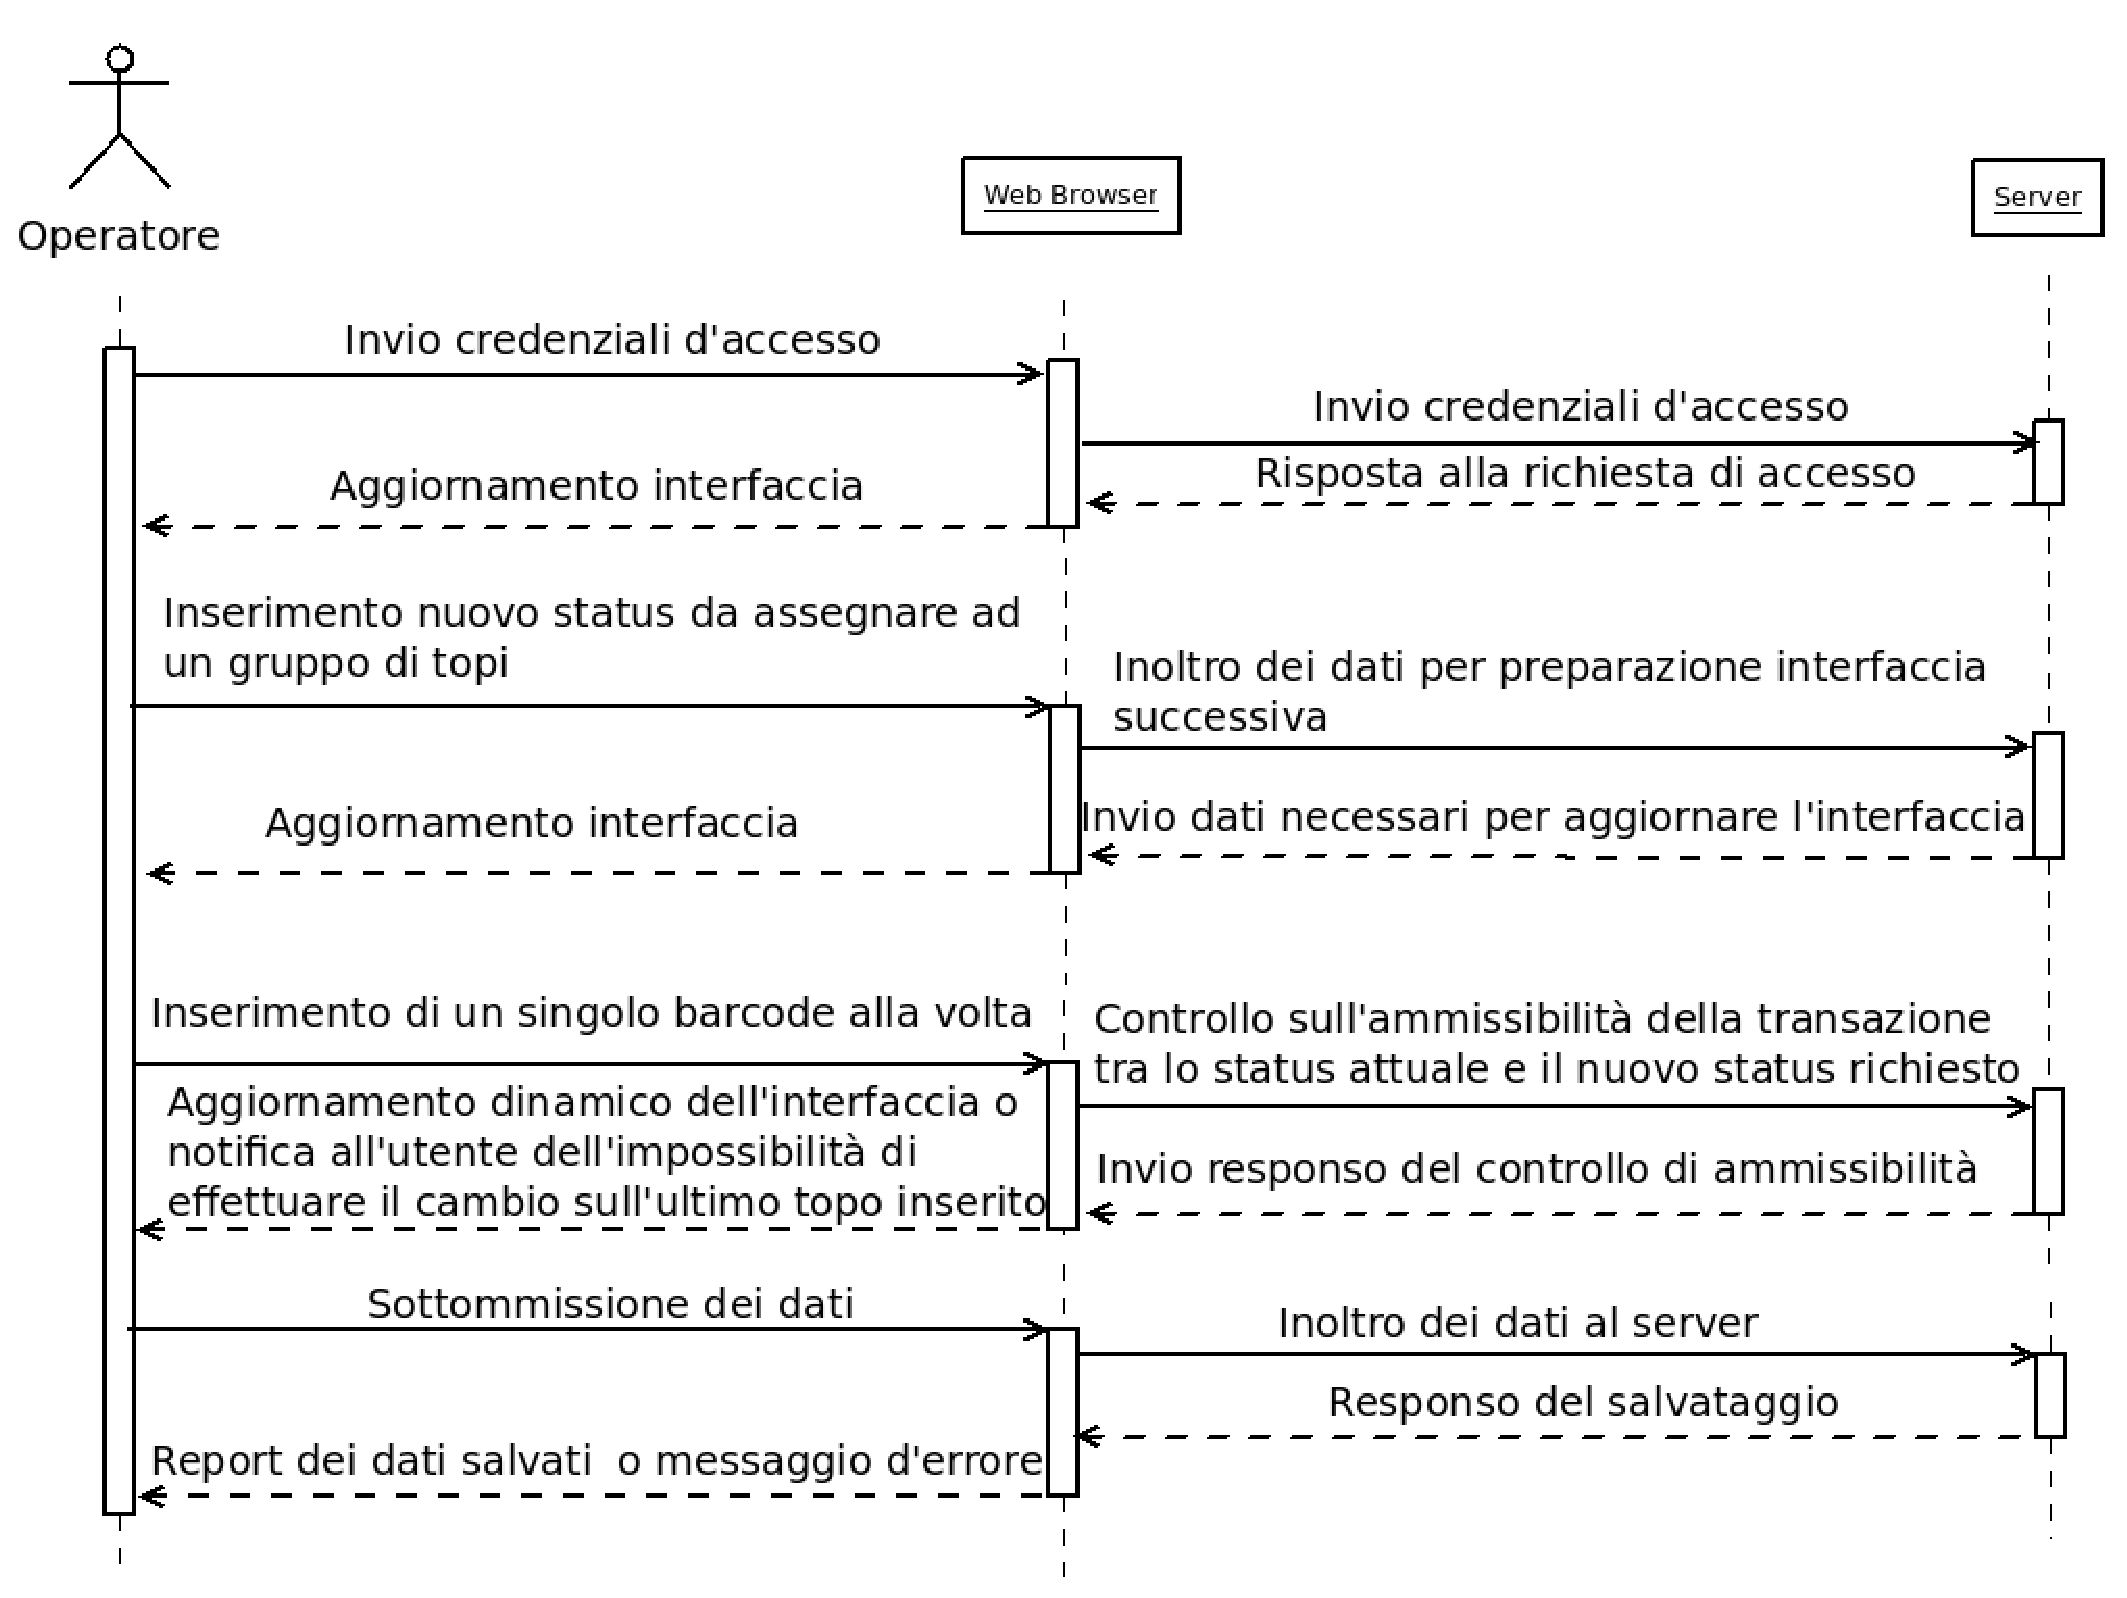
\includegraphics[width=0.6\textwidth]{./Figure/SDchangestatus}
\end{center}
\caption{Diagramma delle sequenze dell'aggiornamento dello status degli xenopazienti\label{fig:SDcs}}
\end{figure}

\newpage

\section{Misurazioni}

In questa Sezione si descrivono le interfacce per la gestione delle misure qualitative e quantitative. Queste due schermate sono molto simili tra di loro, quindi si \`e scelto di descriverle insieme, dettagliando successivamente le singole particolarit\`a. In Figura~\ref{fig:UCDmeasure} \`e riportato il relativo diagramma dei casi d'uso.

\begin{figure}[h]
\begin{center}
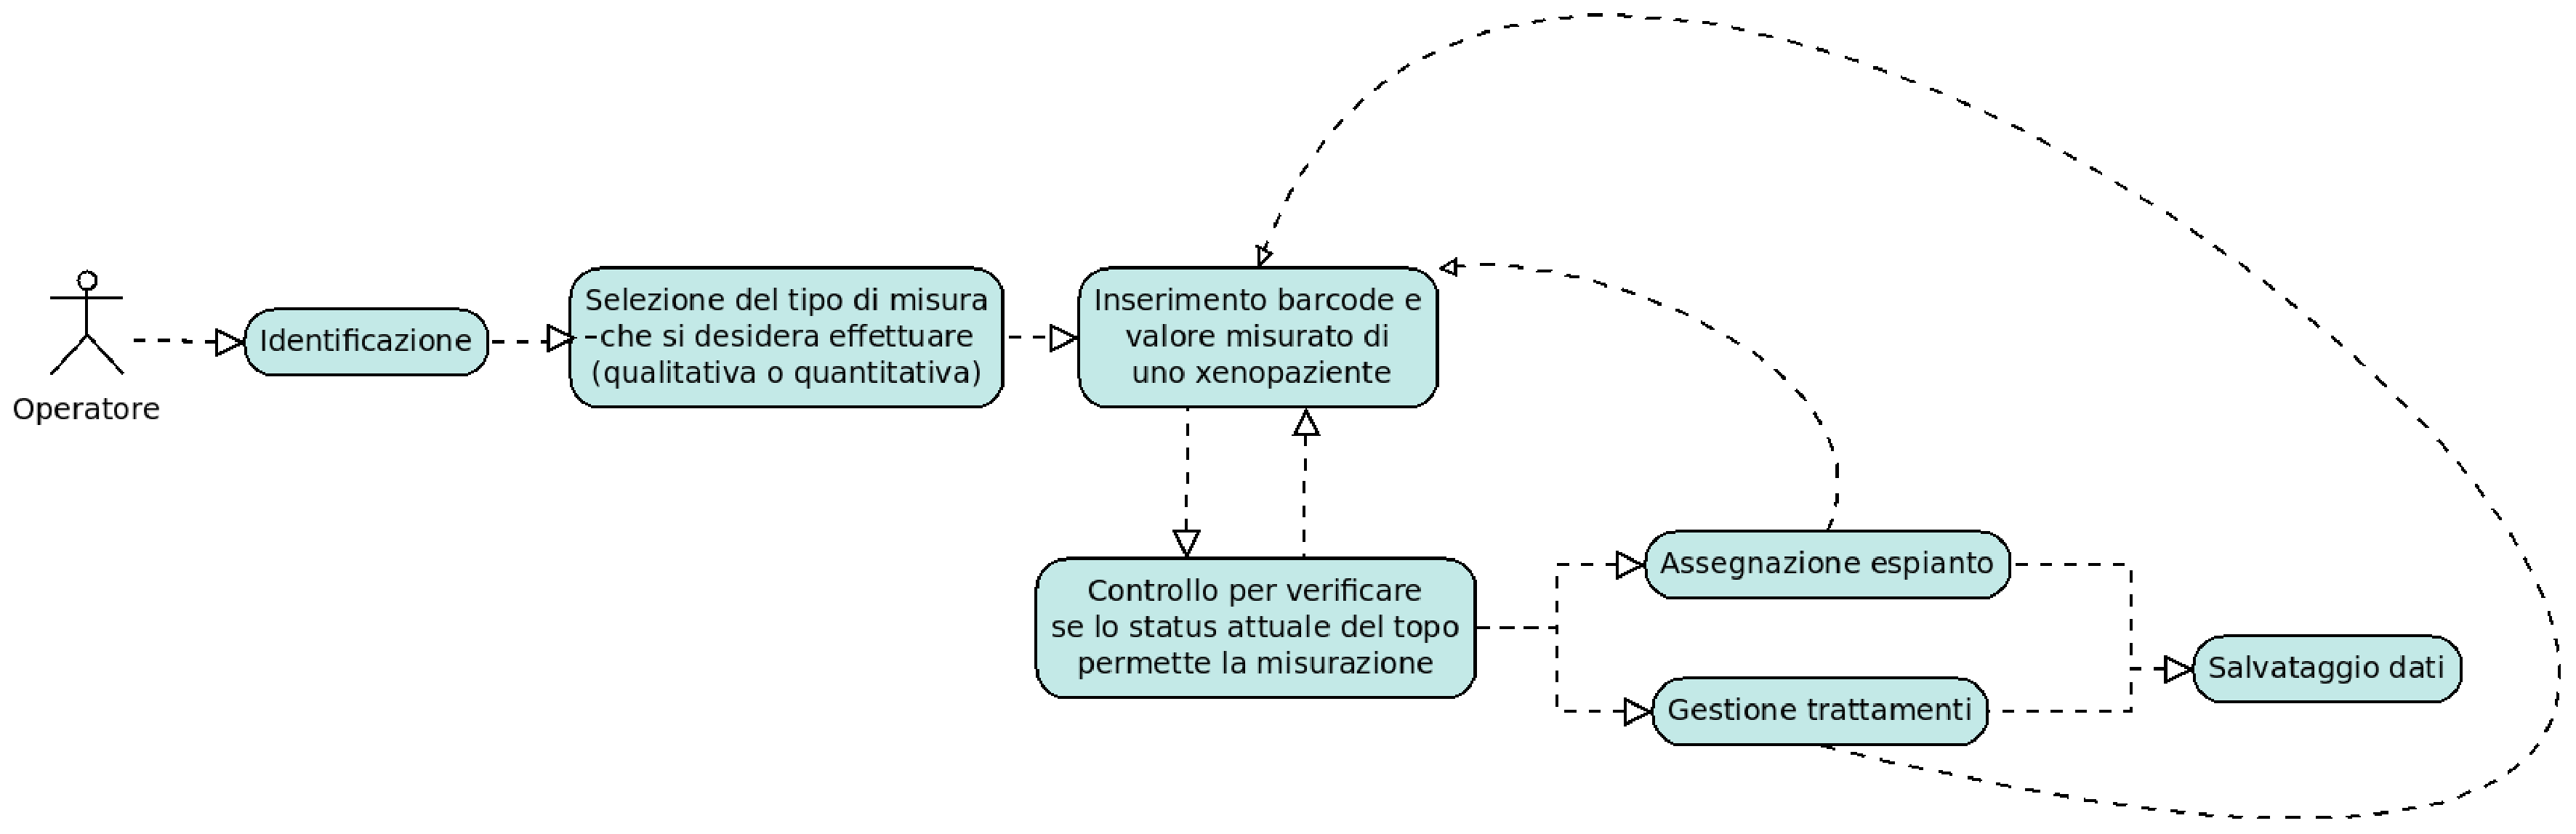
\includegraphics[width=0.9\textwidth]{./Figure/UCDmeasurements}
\end{center}
\caption{UCD delle operazioni di misurazioni\label{fig:UCDmeasure}}
\end{figure}

La somiglianza tra le due interfacce nasce sia perch\`e hanno poche differenze dal punto di vista della loro gestione, sia perch\`e si \`e cercato di mantenere il quanto pi\`u uguali possibili questi due template, per poter dare un ambiente pi\`u familiare all'utente che effettua sia misurazioni di un tipo, sia misurazioni dell'altro.

Nel momento in cui si accede alla schermata delle misurazioni, si specifica il tipo di misure che si vogliono collezionare. Attualmente, le misure consentite sono qualitative e quantitative. L'operatore, dopo aver scelto la tipologia delle misure che si intendono inserire nel database, raggiunge una schermata con una tabella, dove inserire i singoli dati delle varie misurazioni, tramite un apposito form di input. A causa dei vincoli operazionali, in questa tabella si possono inserire solo xenopazienti che hanno lo status \textit{implanted}.

Queste interfacce gestiscono il concetto delle meta-cage, visto nella Sezione~\ref{sec:contrMis}. Da questa tabella, si possono cancellare i topi inseriti, solo tra quelli dell'ultima meta-cage creata.

I campi di testo dove inserire i barcode degli xenopazienti da misurare, sono costruiti in modo tale che, dopo aver ricevuto il barcode dall'apposito lettore, venga automaticamente inserita una riga nell'apposita tabella. Quindi, il barcode \`e l'ultimo dato della misura da inserire, dopo aver immesso il valore relativo. Nel caso di misure quantitative, il valore della misura \`e ricevuto da un apposito calibro elettronico, il quale fornisce i due valori caratterizzanti questo tipo di misura. I campi di testo per questi due valori sono strutturati in modo tale da spostare il focus alla casella di testo successiva dopo aver ricevuto l'input dal calibro. Nella schermata delle misure quantitative, il valore da associare alla misurazione \`e prelevato da un elenco, contenente i dati presenti nella tabella \textit{Qualitative\_values}. Dopo aver inserito una misura di uno xenopaziente, si interroga il database attraverso delle API per verificare se il topo misurato ha un trattamento ad esso associato e se questo \`e acuto, oltre ai dati riguardanti la fine del trattamento stesso. Infine, si recuperano le informazioni su un eventuale espianto programmato sullo xenopaziente in questione.

L'obiettivo di queste due interfacce \`e, oltre a quello di collezionare i dati sulle varie misurazioni, fornire la possibilit\`a di programmare gli espianti sugli xenopazienti. L'espianto \`e programmato a discrezione dell'operatore, dopo che ha valutato la misura effettuata. Inoltre, si svolge anche il compito della gestione dei trattamenti; infatti, da qui si possono gestire i trattamenti sui topi, dopo averli selezionati e cliccando sui tasti per iniziare o fermare un trattamento. L'interfaccia dei trattamenti \`e illustrata nella sezione seguente.

Per le misure quantitave, \`e presente un campo di testo che visualizza la media di tutte le misure inserite nella meta-cage corrente. Inoltre, \`e anche possibile visualizzare la media delle sole righe selezionate, per poter verificare i valori medi di precisi gruppi di xenopazienti. Chiaramente, questo concetto di media non \`e applicabile alle misure qualitative, in quanto si raccolgono valori categorici. Per gestire la media, \`e presente anche un valore di soglia, il quale rappresenta un limite massimo. Nel momento in cui il valore di una media supera questa soglia, le caselle di testo contenenti le due medie si colorano di rosso, in modo tale da fornire un valore pi\`u visibile all'operatore. Per elasticizzare maggiormente il sistema, il valore di soglia \`e modificabile dinamicamente dall'operatore. In Figura~\ref{fig:qm} si pu\`o osservare quanto appena descritto.

\begin{figure}[h]
\begin{center}
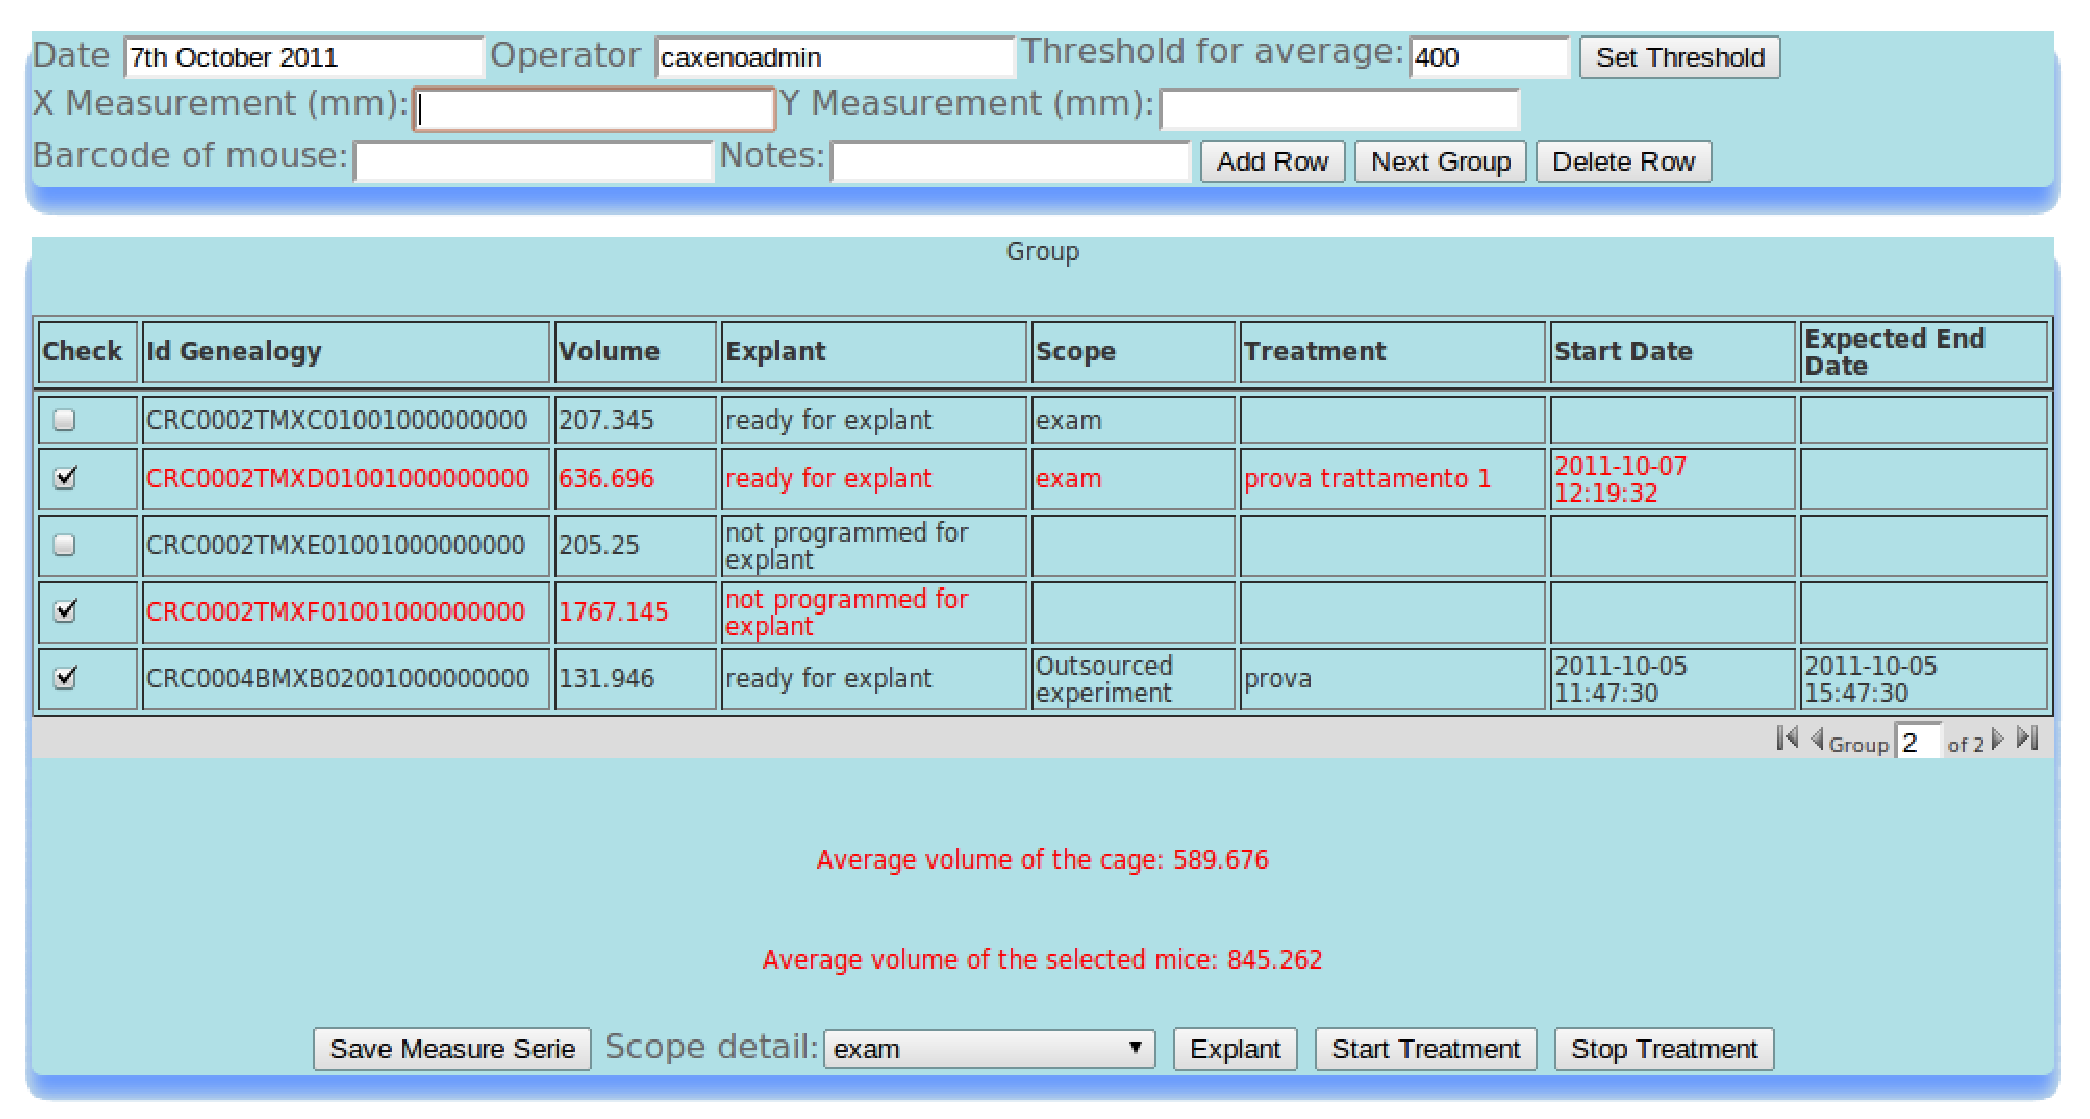
\includegraphics[width=1.0\textwidth]{./Figure/quantMeasure}
\end{center}
\caption{Schermata per la collezione di misure quantitative\label{fig:qm}}
\end{figure}

In Figura~\ref{fig:SDmeasure} si pu\`o osservare il diagramma delle sequenze per la collezione dei dati delle misurazioni.

\begin{figure}[h]
\begin{center}
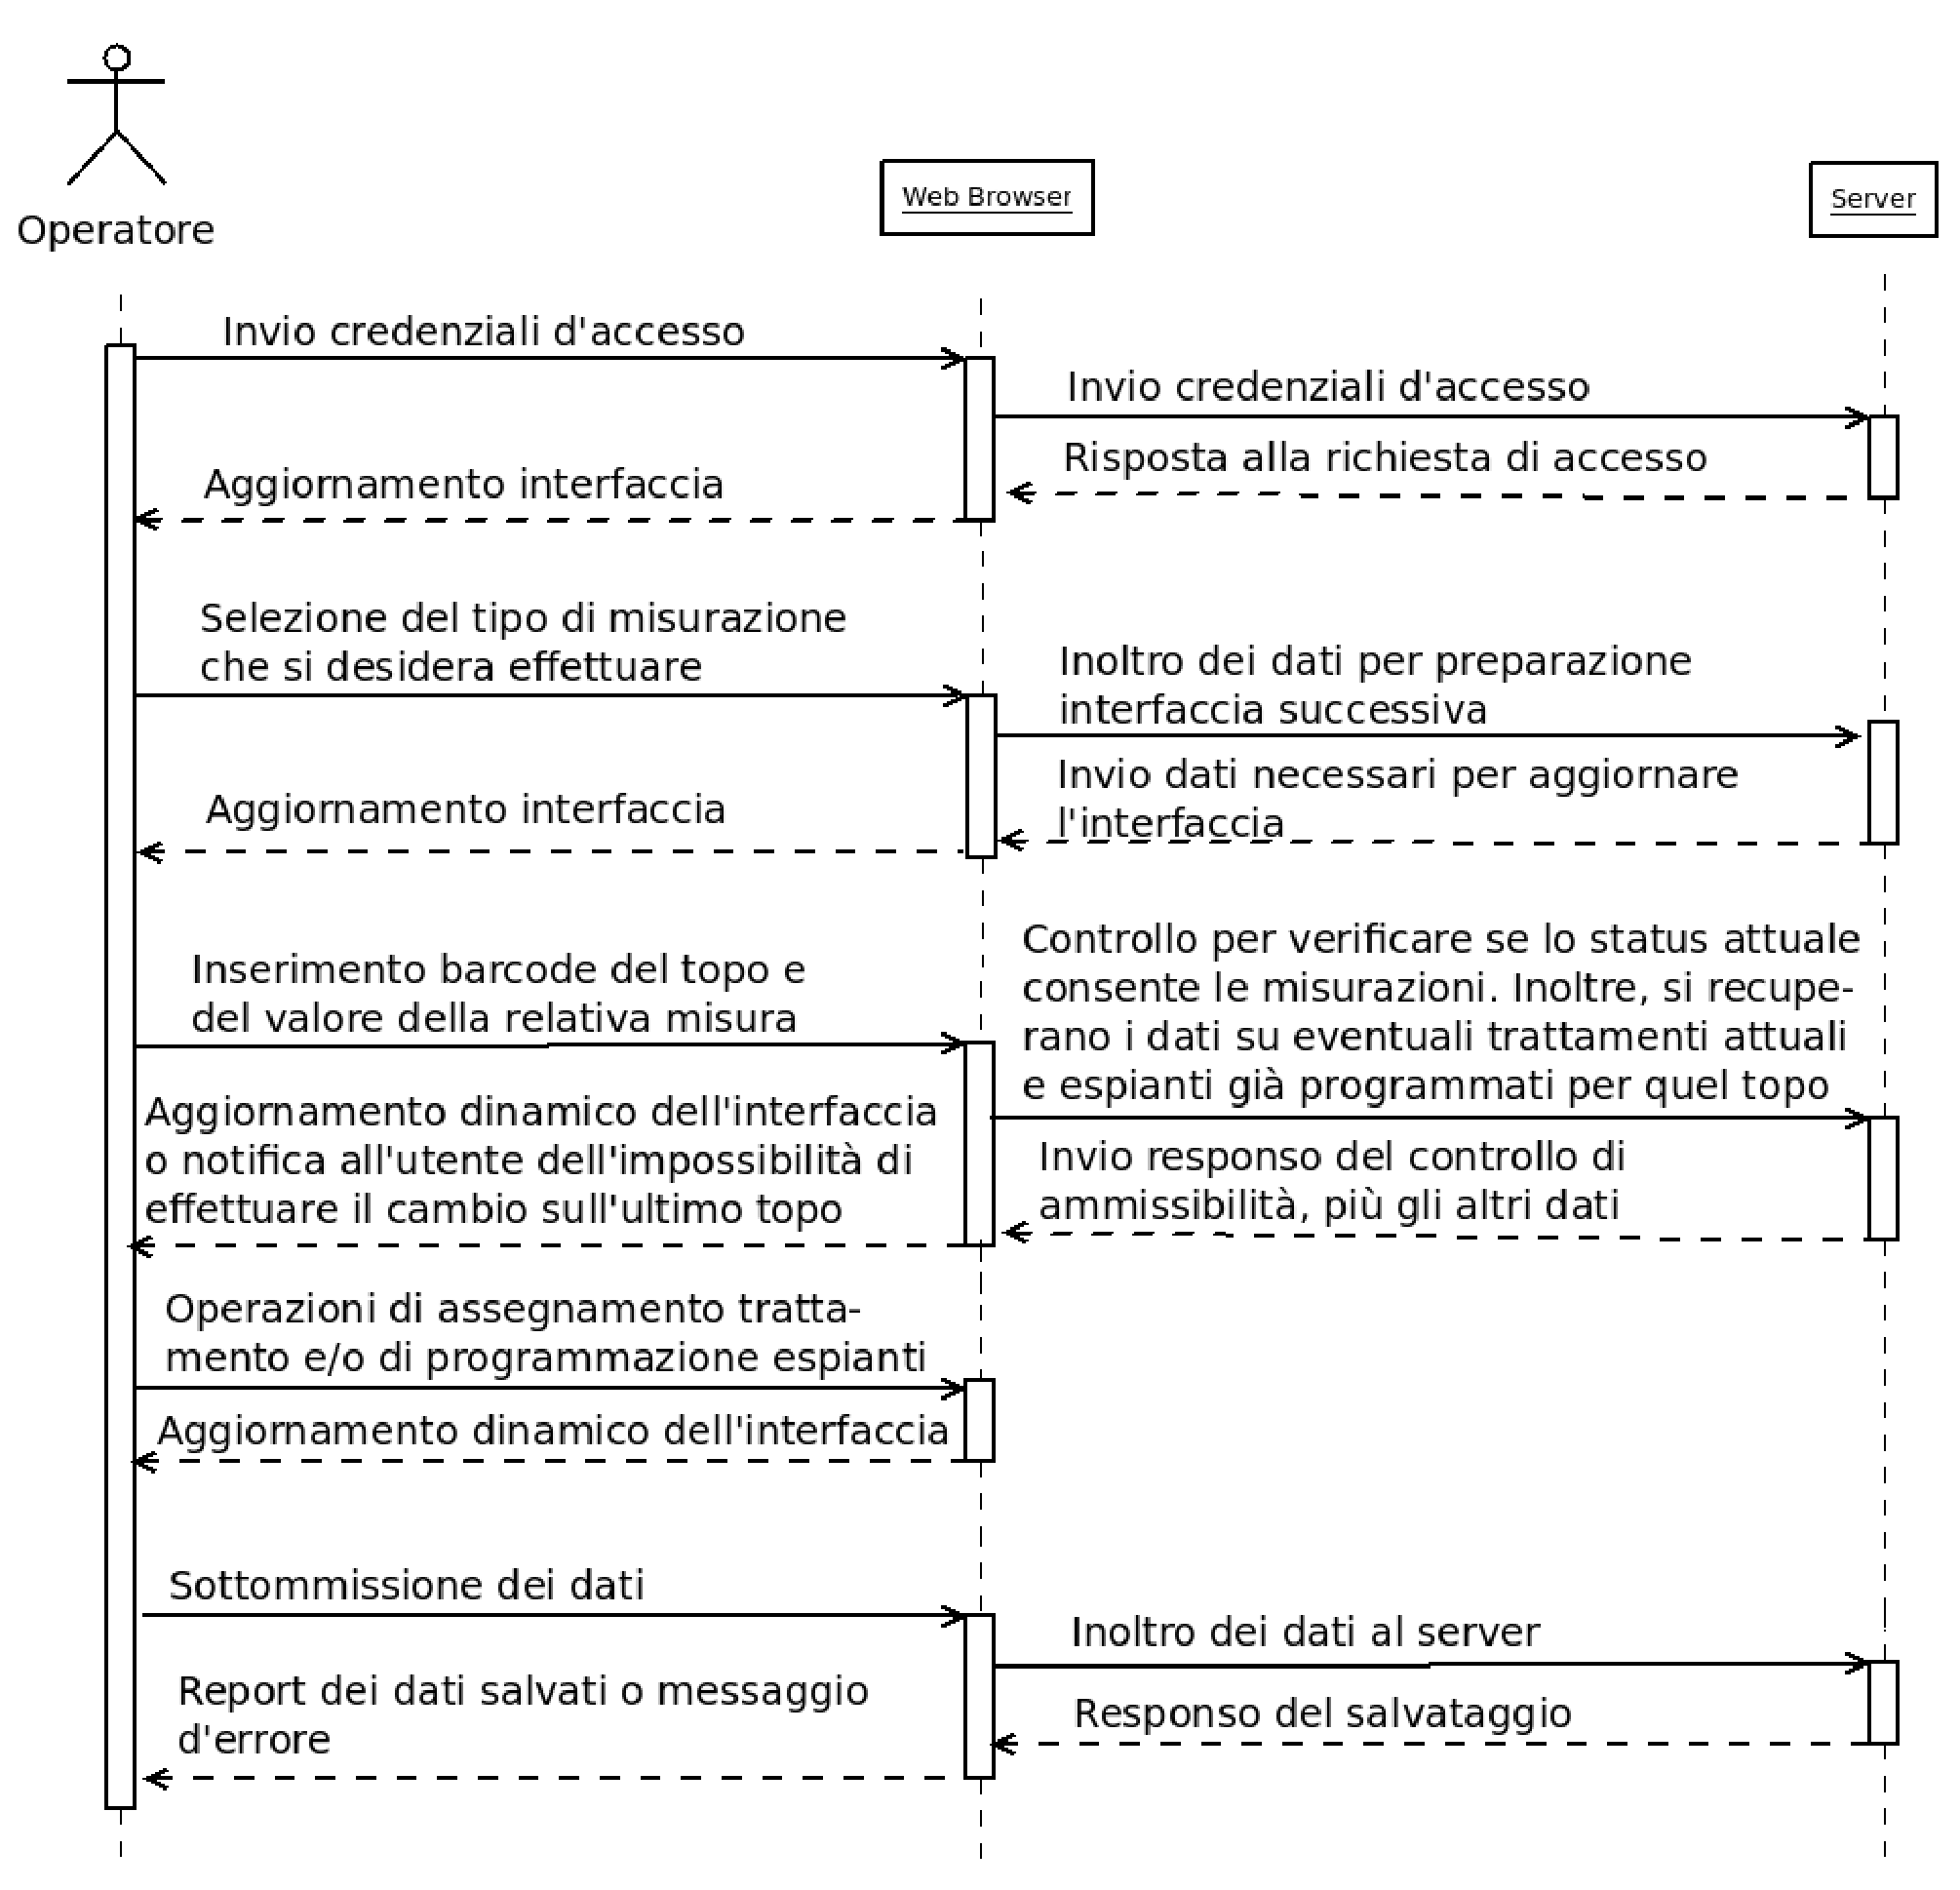
\includegraphics[width=0.6\textwidth]{./Figure/SDmeasurements}
\end{center}
\caption{Diagramma delle sequenze della gestione delle operazioni delle misurazioni\label{fig:SDmeasure}}
\end{figure}

\newpage

\section{Gestione trattamenti}\label{sec:tratt}

Questa interfaccia \`e accessibile solo dopo aver effettuato delle misure su uno o pi\`u xenopazienti. Infatti, dopo averli misurati, se ne seleziona almeno uno dalla tabella, per poi entrare nella finestra per gestire i trattamenti. Sfruttando questo legame con le misurazioni, il diagramma dei casi d'uso dei trattamenti (Figura~\ref{fig:UCDtreat}) pu\`o essere visto come l'espansione del nodo `Gestione trattementi' dell'UCD in Figura~\ref{fig:UCDmeasure}.

\begin{figure}[h]
\begin{center}
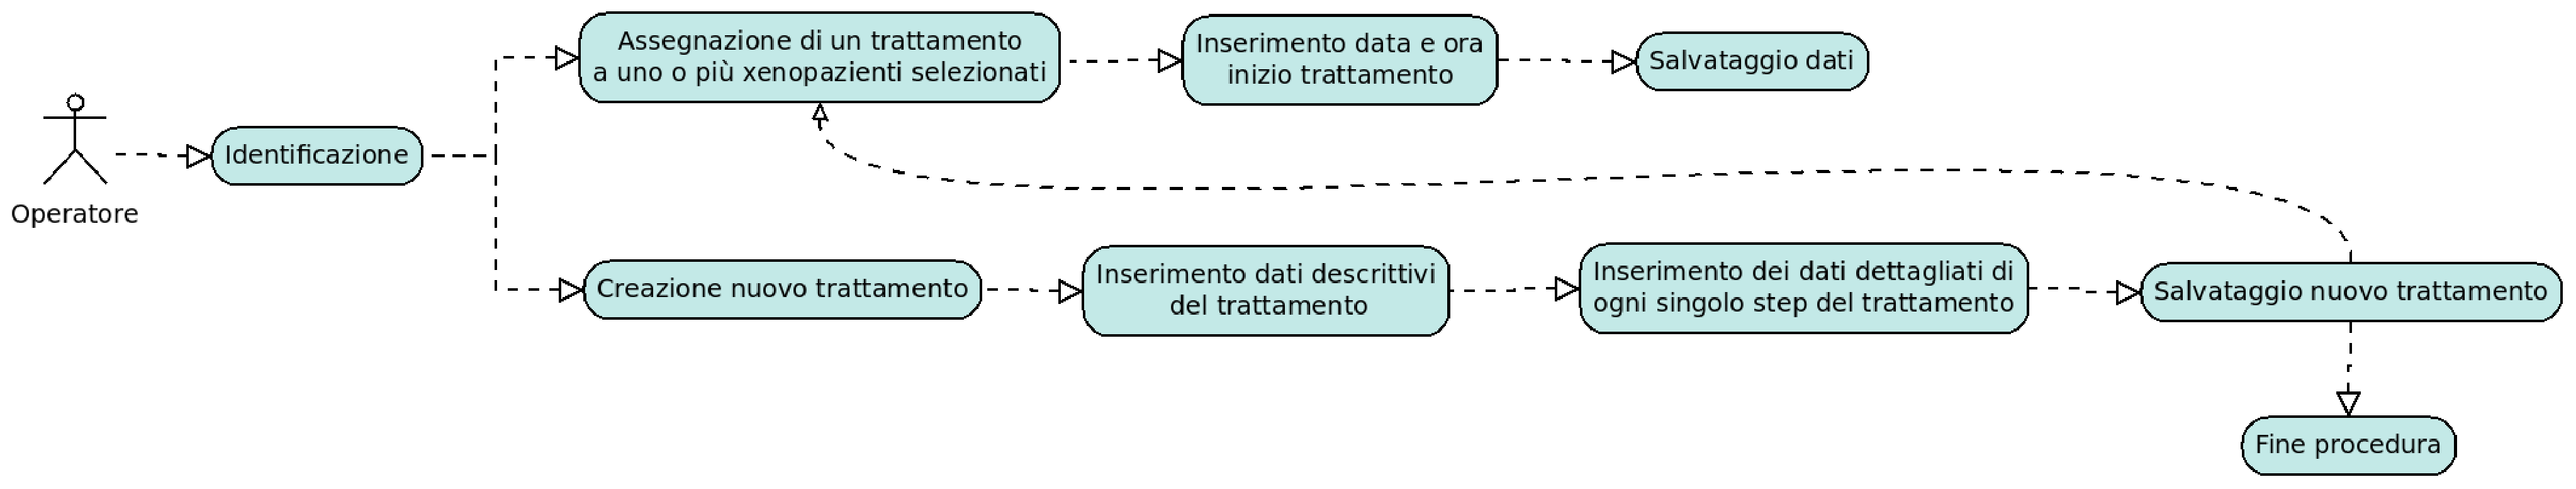
\includegraphics[width=0.9\textwidth]{./Figure/UCDtreatments}
\end{center}
\caption{UCD della gestione dei trattamenti\label{fig:UCDtreat}}
\end{figure}

Nel momento in cui si effettua una misura su uno xenopaziente impiantato, si presenta la possiblit\`a di gestirne i trattamenti. Partendo da ci\`o che offre l'interfaccia, le possibilit\`a sono:
\begin{itemize}
	\item \textbf{avvio trattamento}: si decide di avviare un trattamento su un topo che non ha gi\`a un trattamento in corso. Per sottoporre un topo ad un trattamento, l'utente pu\`o selezionare un trattamento tra quelli esistenti oppure crearne uno ad hoc, rendendolo cos\`i disponibile per eventuali usi futuri. \`E possibile quindi applicare pi\`u volte lo stesso trattamento a diversi topi, in modo tale da poter confrontare i risultati sperimentali ottenuti su soggetti diversi;
	\item \textbf{interruzione trattamento}: se si reputa inutile il proseguimento di un trattamento, lo si pu\`o interrompere prima della sua scadenza programmata. Questa operazione \`e svolta senza accedere direttamente all'interfaccia creata per la gestione delle misurazioni;
	\item \textbf{stop\&start trattamento}: questa possibilit\`a \`e la combinazione delle due precedenti, utilizzata nel caso in cui si voglia applicare un trattamento diverso da quello attuale.
\end{itemize}

Per avviare un nuovo trattamento, si accede all'apposita interfaccia. Per scegliere il trattamento da cominciare, si accede ad un elenco di trattamenti disponibili. Inoltre si ha la possibilit\`a di scegliere quando farlo cominciare. Se in questa lista non \`e presente ci\`o che si desidera, si avvia la procedura per crearne uno nuovo, per poi assegnarlo agli xenopazienti precedentemente selezionati.

Nel momento in cui si crea un nuovo trattamento, se ne inseriscono i dati descrittivi, quali il nome, una breve descrizione, la durata e la tipologia di trattamento a cui appartiente. Il nome assegnato al nuovo trattamento deve essere univoco. Per assicurare questo vincolo, si \`e implementato un'apposita API per verificare i dati gi\`a presenti nel database. Le tipologie dei trattamenti sono, attualmente, due: i trattementi base e i trattamenti acuti. Questi ultimi hanno la particolarit\`a che, una volta interrotti o terminati, implicano un espianto forzato degli xenopazienti sui quali \`e stato applicato.

Specificare la durata e la sua unit\`a di misura, serve per creare, successivamente, il diagramma di Gantt (strumento di supporto alla gestione dei progetti\cite{gantt}) per programmare nel dettaglio i vari passaggi del trattamento che si sta creando. L'utente pu\`o dinamicamente aggiungere varie righe, dove ognuna di questa rappresenta un determinato passaggio del trattamento, caratterizzato dal farmaco e dal modo in cui viene somministrato, dalla dose e dal numero di volte che deve essere utilizzato nell'unit\`a di tempo precedentemente selezionata (ad esempio, 2 volte ogni ora o 1 al giorno), dove ogni colonna costituisce uno slot temporale, come illustrato in Figura~\ref{fig:gantt}. Dopo aver inserito le righe desiderate, ci si ritrova con una tabella dove ogni cella corrisponde a una determinata somministrazione in un certo slot temporale. Selezionando le celle, si pu\`o cos\`i creare un trattamento composto da molteplici step molto dettagliati. Se si sbaglia ad inserire una riga, \`e sufficiente lasciarla vuota per fare in modo che non venga salvata nel database. Una volta salvato il trattamento, e dopo aver ricevuto un messaggio di conferma, si torna alla schermata precedente, dove si pu\`o ora selezionare il nuovo trattamento ed assegnarlo agli xenopazienti. In Figura~\ref{fig:SDtreat} si pu\`o osservare il diagramma delle sequenze di questa interfaccia.

\begin{figure}[h]
\begin{center}
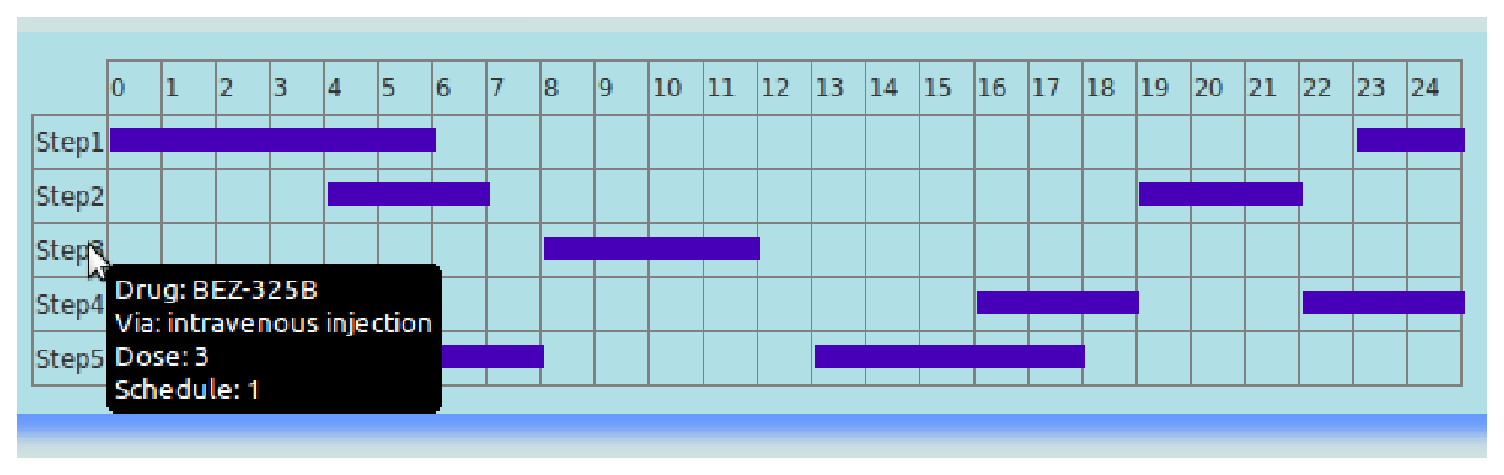
\includegraphics[width=1.0\textwidth]{./Figure/gantt}
\end{center}
\caption{Esempio di utilizzo del diagramma di Gantt in XMS\label{fig:gantt}}
\end{figure}

\begin{figure}[h]
\begin{center}
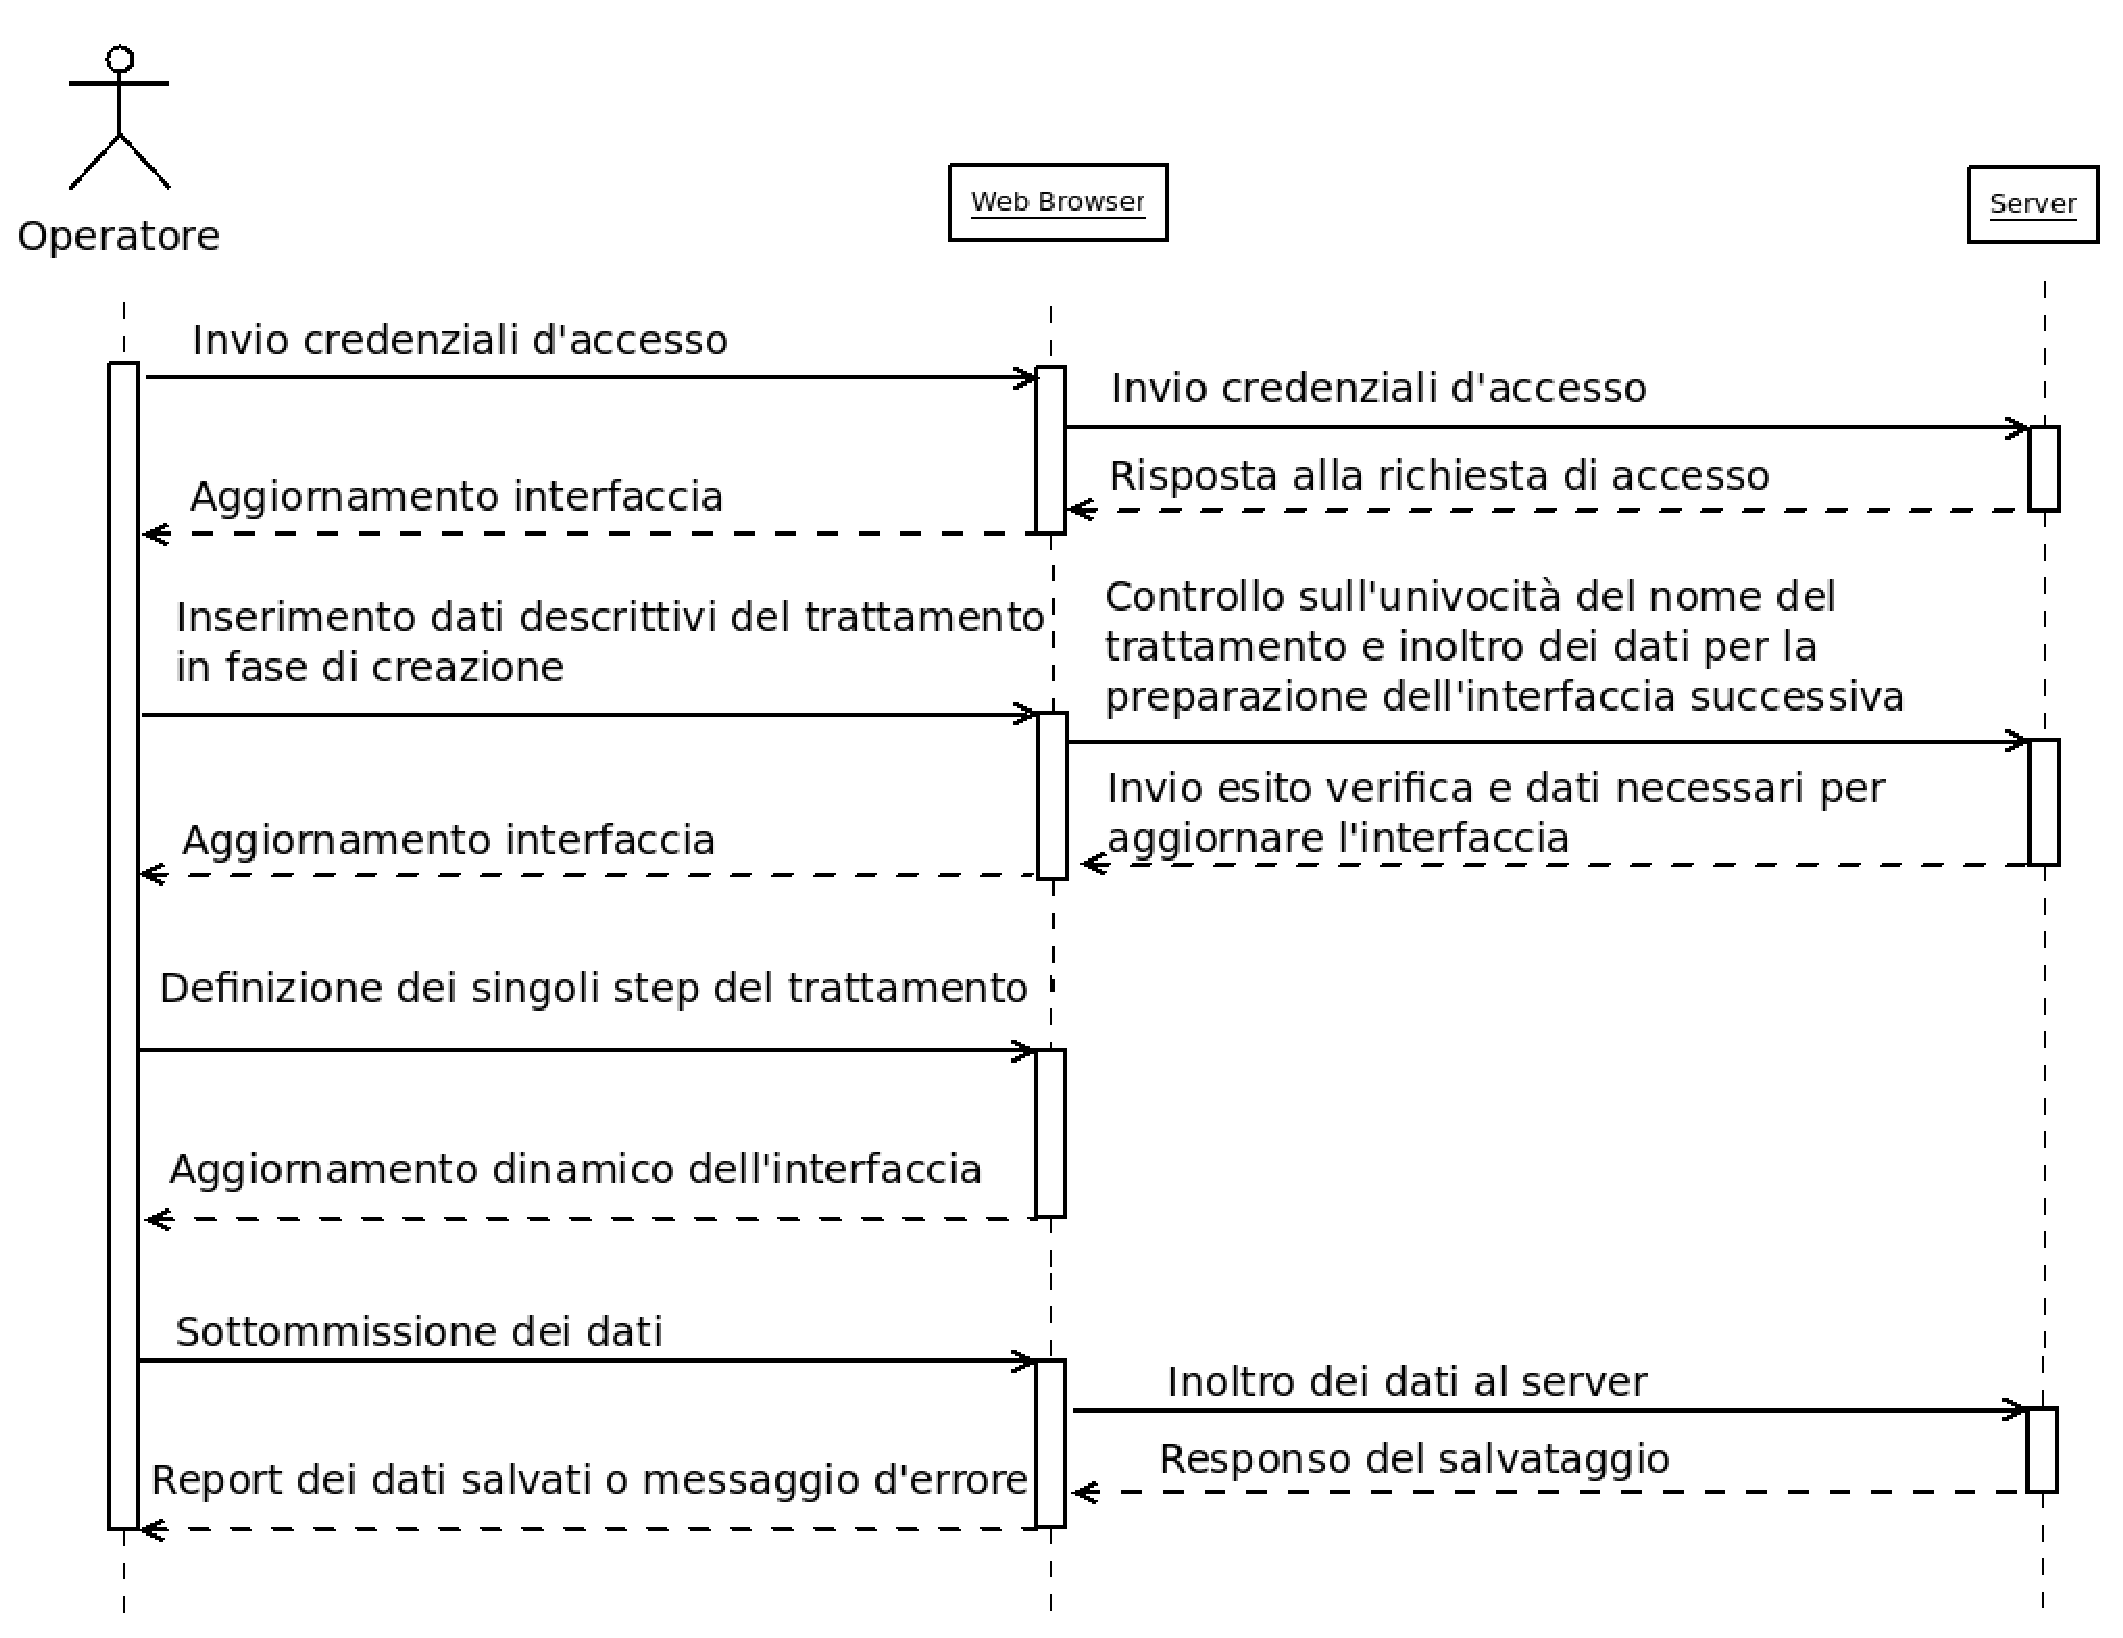
\includegraphics[width=0.6\textwidth]{./Figure/SDtreatmentsCreate}
\end{center}
\caption{Diagramma delle sequenze delle operazioni effettuate per creare un trattamento\label{fig:SDtreat}}
\end{figure}

\newpage

\section{Impianti}

Considerando l'ordine temporale delle operazioni svolte su uno xenopaziente nel suo ciclo di vita, la gestione degli impianti \`e la prima dove si \`e cercato di simulare l'ambiente di laboratorio. In Figura~\ref{fig:UCDimpl} \`e riportato il diagramma dei casi d'uso relativo a questa interfaccia.

\begin{figure}[h]
\begin{center}
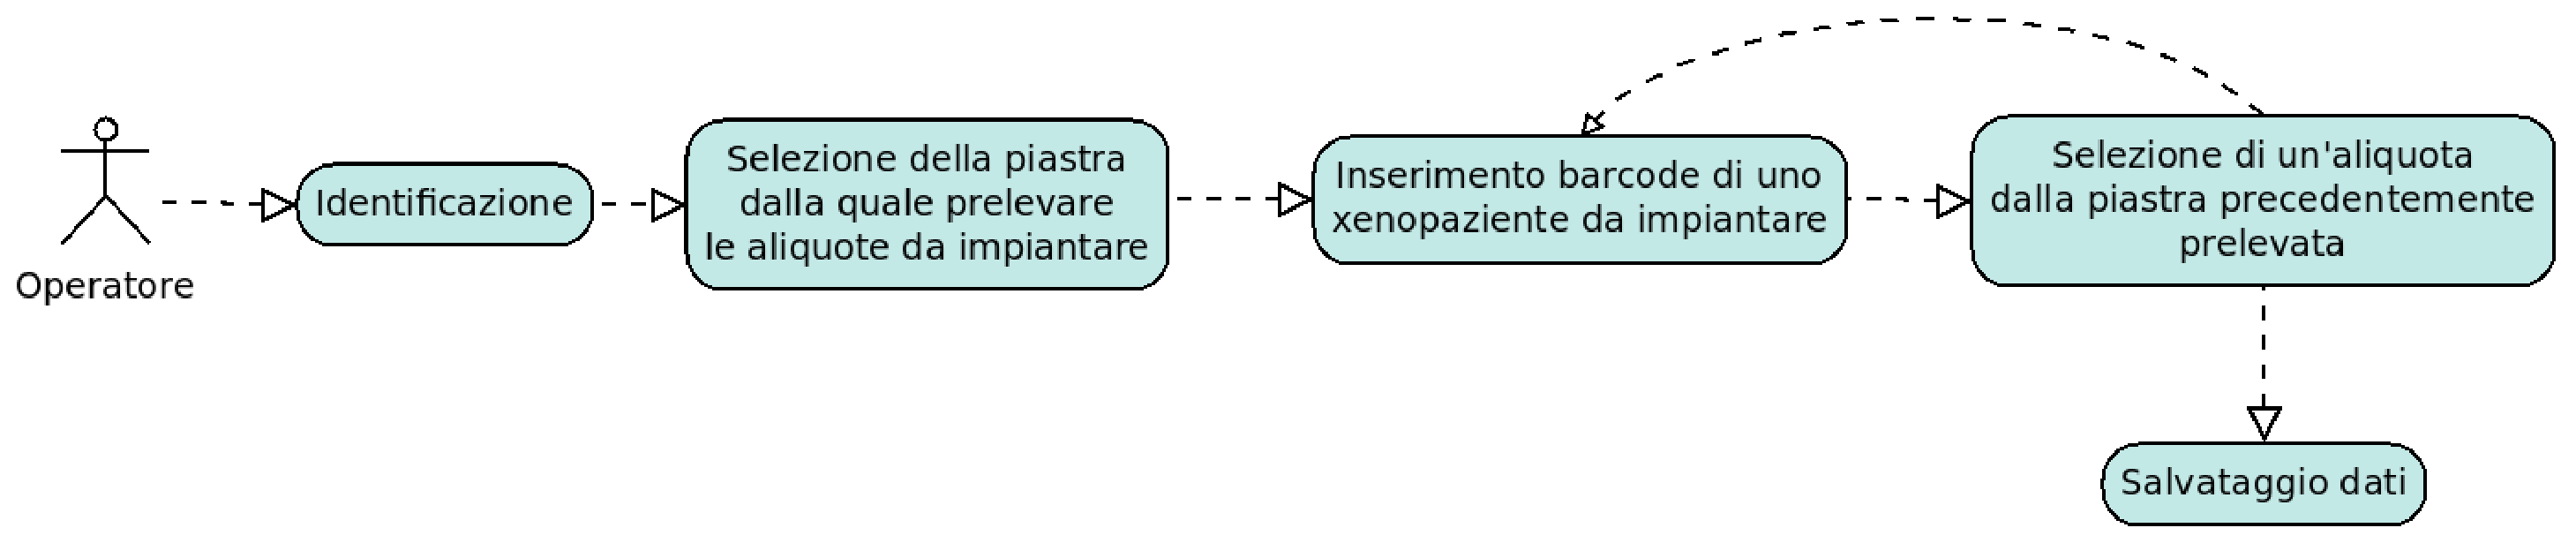
\includegraphics[width=0.8\textwidth]{./Figure/UCDimplants}
\end{center}
\caption{UCD relativo agli impianti\label{fig:UCDimpl}}
\end{figure}

Nel database, le informazioni relative ad un determinato insieme di impianti sono tra loro collegate tramite una serie, conetto utilizzato per raggruppare gli impianti svolti nella stessa sessione operativa (stessa piastra sorgente, data e operatore). Anche l'utente \`e cosciente di questo concetto, grazie alla struttura con la quale \`e stata costruita l'interfaccia degli impianti. Infatti, prima di inserire i dettagli di ogni singola operazione, vengono richiesti i dati comuni a tutta la serie di operazioni: la data dell'impianto e un eventuale commento. Inoltre, molto importante, si inserisce il barcode della piastra dalla quale si intendono prelevare le aliquote da impiantare. Questo barcode viene inoltrato alla BioBanaca, la quale, tramite apposite API, invia al \Xeno\ le informazioni riguardanti la piastra richiesta e le aliquote eventualmente contenute in essa. Grazie a questo scambio di informazioni, si \`e in grado di costruire un tabella che simula la piastra e la disposizione delle provette all'interno di essa, dalla quale l'utente pu\`o selezionare l'aliquota da impiantare nel topo. Dopo aver inserito i dati preliminari, si accede alla schermata nella quale definire i singoli impianti. In questa interfaccia possono essere utilizzati solo xenopazienti aventi lo status \textit{experimental}. Se si cerca di utilizzare un topo che non appartiente a questo status, si notifica un messaggio all'operatore.

Per la simulazione della piastra, \`e stata creata una tabella rappresentante una piastra, dove ogni cella simula una provetta, contenente una determinata aliquota. Si \`e inserito un numero per ogni cella, rappresentante la quantit\`a di frammenti della stessa aliquota presente in quella provetta. Inoltre, \`e stato implementato un sistema cromatico, con un colore associato ad ogni cella, per poter visionare velocemente la situazione della piastra. In Figura~\ref{fig:implantP} se ne pu\`o vedere un esempio, mentre di seguito si elencano e descrivono i colori utilizzati:
\begin{enumerate} 
  \item giallo chiaro: \`e presente almeno un'aliquota nella provetta rappresentata da questa cella;
  \item nero: non \`e presenta alcuna aliquota;
  \item giallo scuro: sono finite le aliquote inizialmente presenti in quella cella;
  \item azzurro: l'aliquota \`e attualmente selezionata.
\end{enumerate} 

\noindent Appena \`e selezionata un'aliquota, nella pagina viene visualizzato il suo identificativo di genealogia e il nuovo identificativo di genealogia da essa creato, che sar\`a assegnato allo xenopaziente impiantato con quel tessuto.

\begin{figure}[h]
\begin{center}
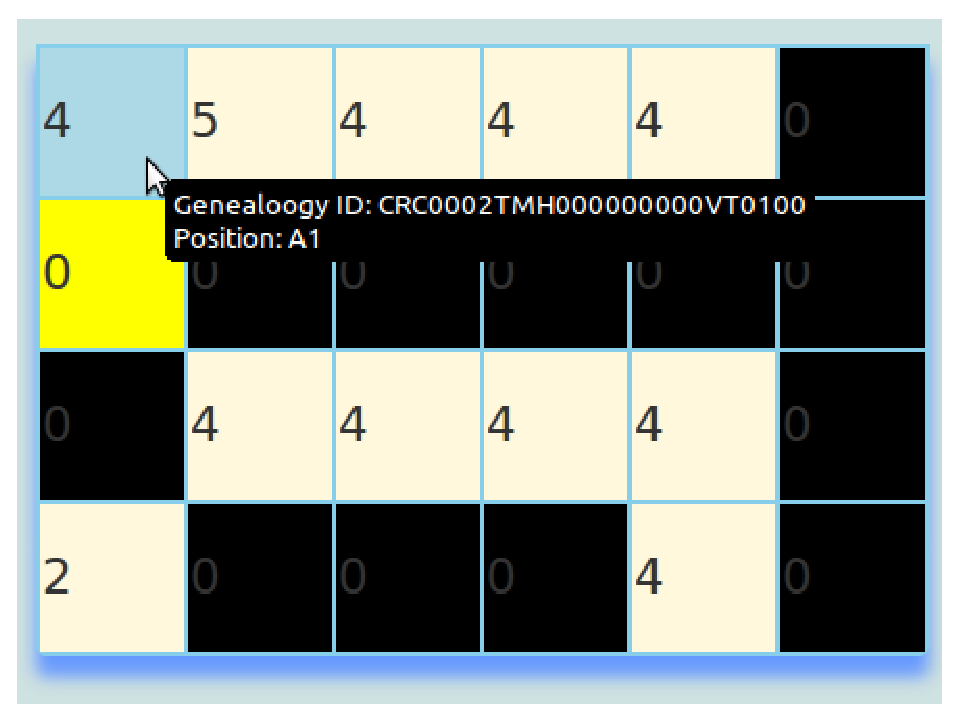
\includegraphics[width=0.6\textwidth]{./Figure/implantPlate}
\end{center}
\caption{Utilizzo della tabella contenente i dati delle aliquote\label{fig:implantP}}
\end{figure}

Oltre a selezionare l'aliquota, si deve anche selezionare il topo, il sito dell'impianto e settare eventualmente il BadQualityFlag (il quale indica un impianto mal riuscito). Una volta selezionati sia l'aliquota, sia lo xenopaziente (non necessariamente in questo ordine), si pu\`o procedere ad inserire l'impianto appena impostato nella tabella riepilogativa, dalla quale, in caso di errore, si possono cancellare le righe relative alle operazioni errate. Quando l'inserimento dati \`e terminato, si pu\`o completare la serie di impianti cliccando su `Save'. Se la piastra impiegata ha ancora aliquote al suo interno, si chiede all'utente se si desidera svuotarne il contenuto. Dopodich\`e, in caso di esito positivo della transazione, si visualizza il report dei dati appenna immessi nel database. Inoltre, si invia la lista delle aliquote utilizzate alla \Tissue\ e l'informazione relativa all'eventuale svuotamento della piastra. In Figura~\ref{fig:SDimpl} si pu\`o osservare il diagramma delle sequenze di questa interfaccia.

\begin{figure}[h]
\begin{center}
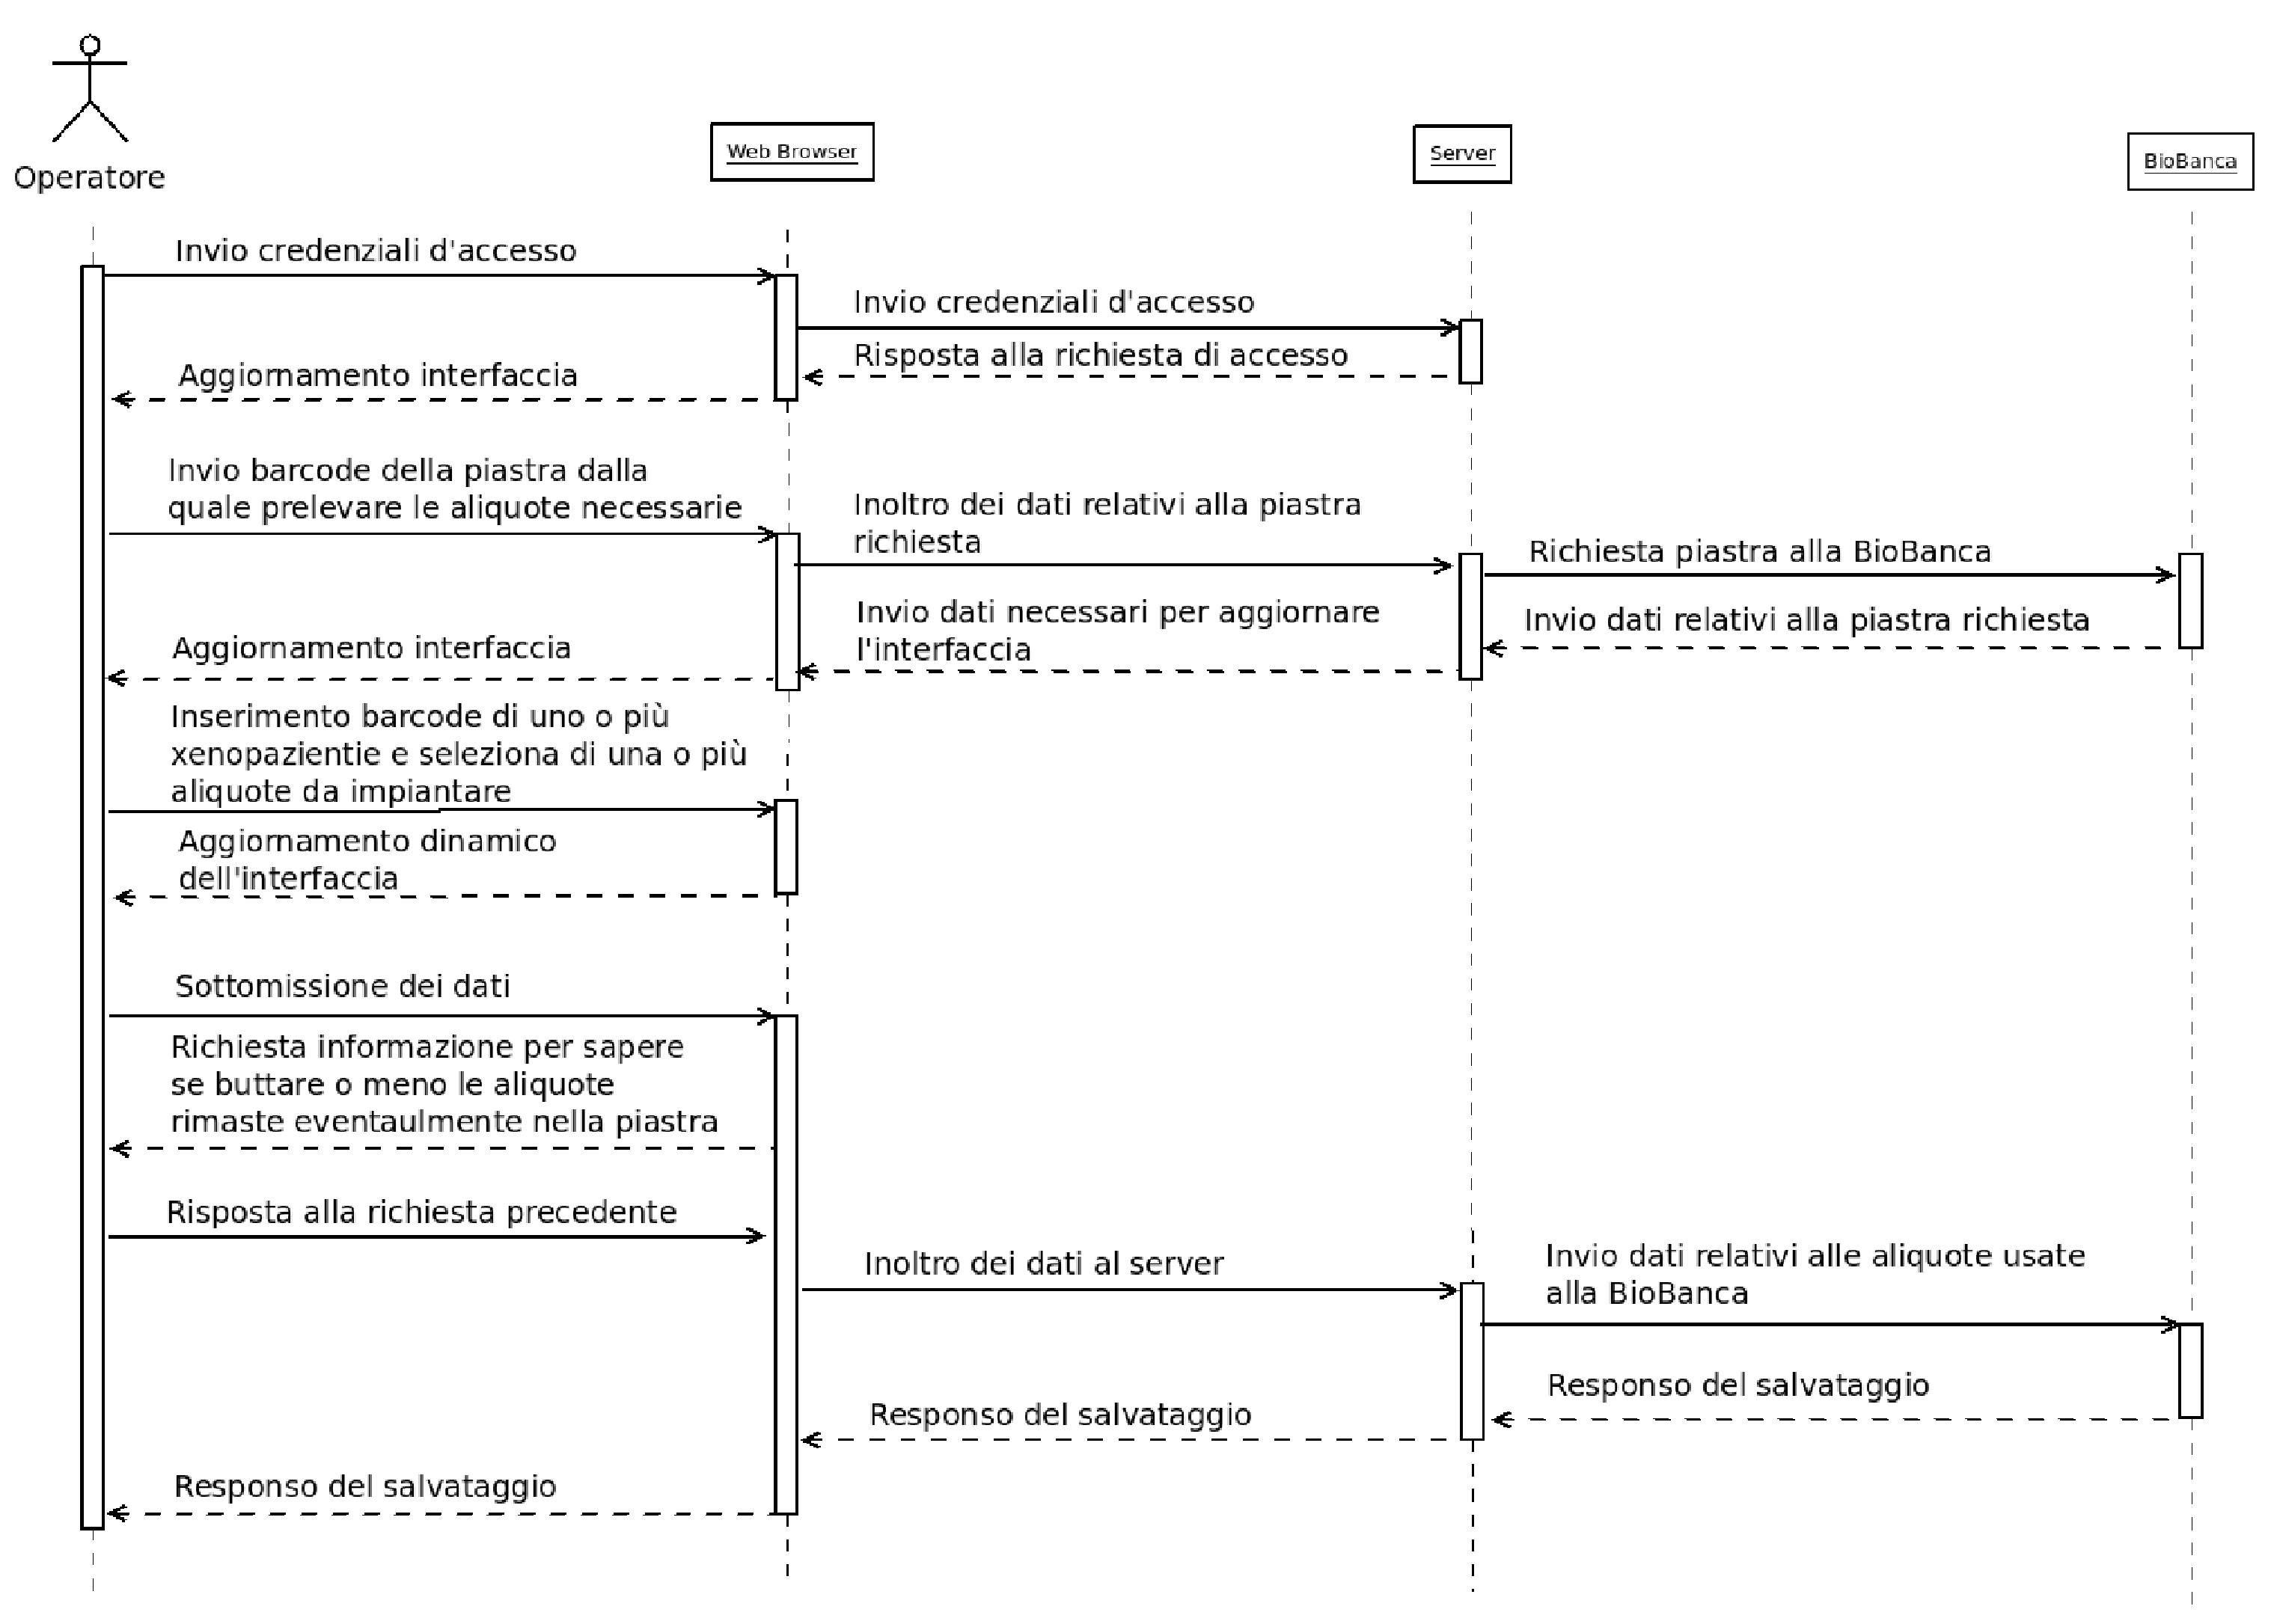
\includegraphics[width=0.9\textwidth]{./Figure/SDimplants}
\end{center}
\caption{Diagramma delle sequenze delle operazioni effettuate per creare un trattamento\label{fig:SDimpl}}
\end{figure}

\newpage

\section{Espianti}

Nel momento in cui si desidera effettuare una serie di espianti, per collezionare del materiale, si deve utilizzare una prima schermata preliminare, per selezionare i dati da elaborare nella pagina successiva. In questa prima interfaccia, si accede all'elenco degli \textit{xenopazienti} sui quali \`e stato programmato un espianto. Oltre a selezionare uno o pi\`u topi di questa lista, si devono anche selezionare i tipi di tessuto che si intendono generare durante l'espianto, in modo tale da poter gestire pi\`u efficacemente la schermata successiva. Un'ultimo parametro da introdurre \`e la data in cui viene effettuata questa operazione (la data di default \`e quella odierna). Questi dati preliminari consentono di inserire nel database le informazioni relative alla serie di espianti che si va a effettuare. In Figura~\ref{fig:UCDexpl} \`e riportato il diagramma dei casi d'uso relativo a questa interfaccia.

\begin{figure}[h]
\begin{center}
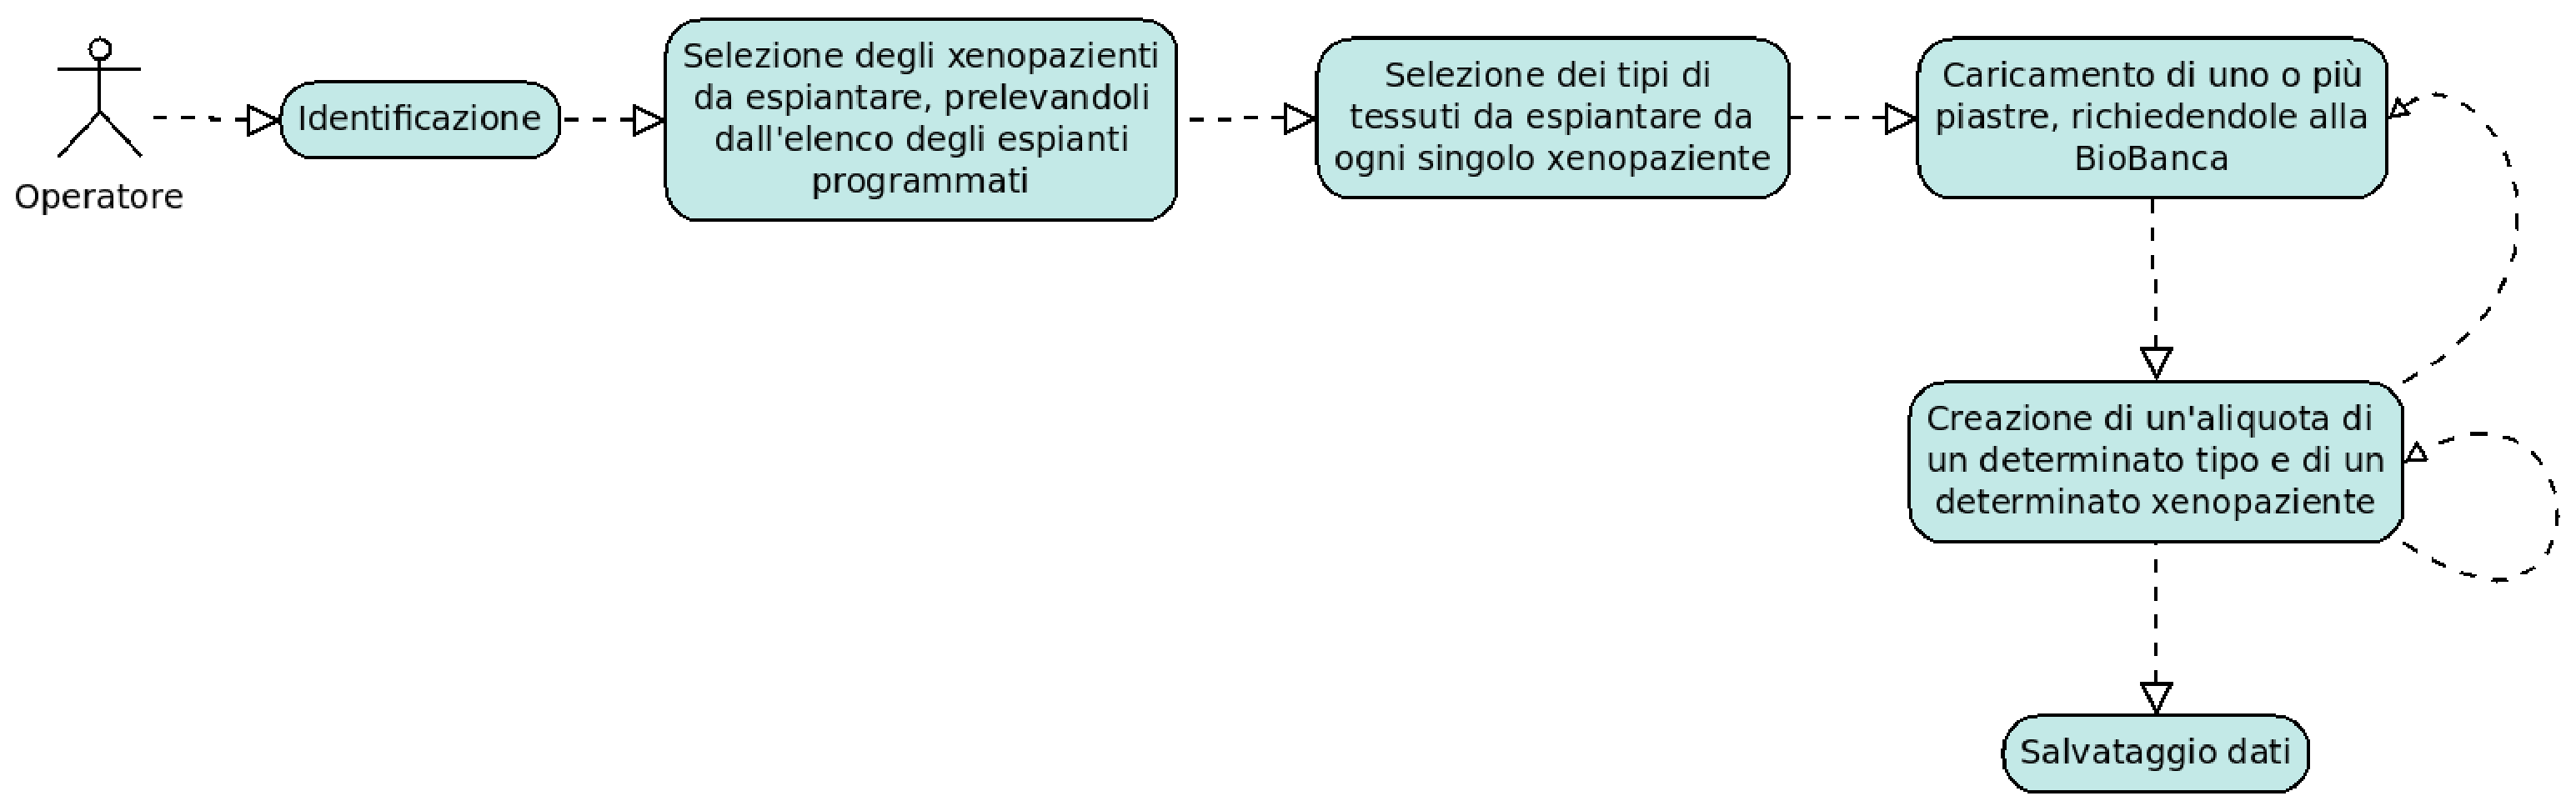
\includegraphics[width=0.8\textwidth]{./Figure/UCDexplants}
\end{center}
\caption{UCD relativo agli espianti\label{fig:UCDexpl}}
\end{figure}

Dopo aver visionato e selezionati gli xenoapazienti che si intendono espiantare, si accede ad un'interfaccia per gestire la collezione di nuovo materiale biologico. Questa schermata \`e stata costruita con l'intento di simulare l'ambiente di laboratorio. Questo rende agevole l'impatto con questa interfaccia agli addetti ai lavori, i quali conoscono bene le procedure di studio e ricerca.

Durante l'espianto, l'operatore pu\`o destinare le aliquote prelevate dal topo, in diversi tipi di provette, a loro volta contenute in diverse categorie di piastre (una piastra \`e un supporto in grado di contenere diverse provette al suo interno). Per simulare questa possibilit\`a di scelta, si \`e creata una tabella per ogni tipologia di piastra, dove ogni cella rappresenta una provetta in cui depositare il tessuto ottenuto dall'espianto appena eseguito. Le diverse piastre rispondono alla necessit\`a di avere diversi tipi di conservazione dei tessuti. Questa interfaccia, presentatata nella Figura~\ref{fig:explForm}, offre sei tabelle, ognuna rappresentante una diversa procedura per conservare il materiale:
\begin{itemize}
	\item \textbf{vital}: le aliquote vengono tenute un giorno in congelatore a -80\textcelsius\ e poi conservate in azoto liquido a -196\textcelsius;
	\item \textbf{snap frozen}: si effettua un rapido congelamento attraverso l'impiego di azoto liquido, per poi conservare le aliquote a -80\textcelsius;
	\item \textbf{RNAlater}: il tessuto \`e immerso in una soluzione acquosa per stabilizzare e proteggere i tessuti freschi, senza avere l'obbligo della conservazione in un congelatore (anche se cos\`i si aumenta il tempo per il quale l'aliquota pu\`o essere conservata). La soluzione acquosa \`e un fissativo blando e serve soprattutto per conservarre gli acidi nucleici. Vengono tenuti in frigo per 24h e poi congelati a -80\textcelsius;
	\item \textbf{formalin fixed}: i frammenti di tessuto vengono fissati per 24h in una soluzione contenente formalina e poi inclusi in un blocco di paraffina al fine di conservarli a temperatura ambiente (\`e il classico metodo di archiviazione utilizzato negli ospedali);
	\item \textbf{OCT frozen}: l'aliquota viene inglobata in una particolare resina chiamata OCT, che solidifica a basse temperature. Successivamente, si conserva in freezer, a -80\textcelsius;
	\item \textbf{ChinaBlack}: il tessuto viene insufflato con una soluzione di nero di china in modo da far risaltare eventuali metastasi come punti chiari su un fondo nero. Il materiale viene poi conservato a temperatura ambiente in una soluzione fissativa a base di metanolo e formaldeide. 
\end{itemize}

\begin{figure}[h]
\begin{center}
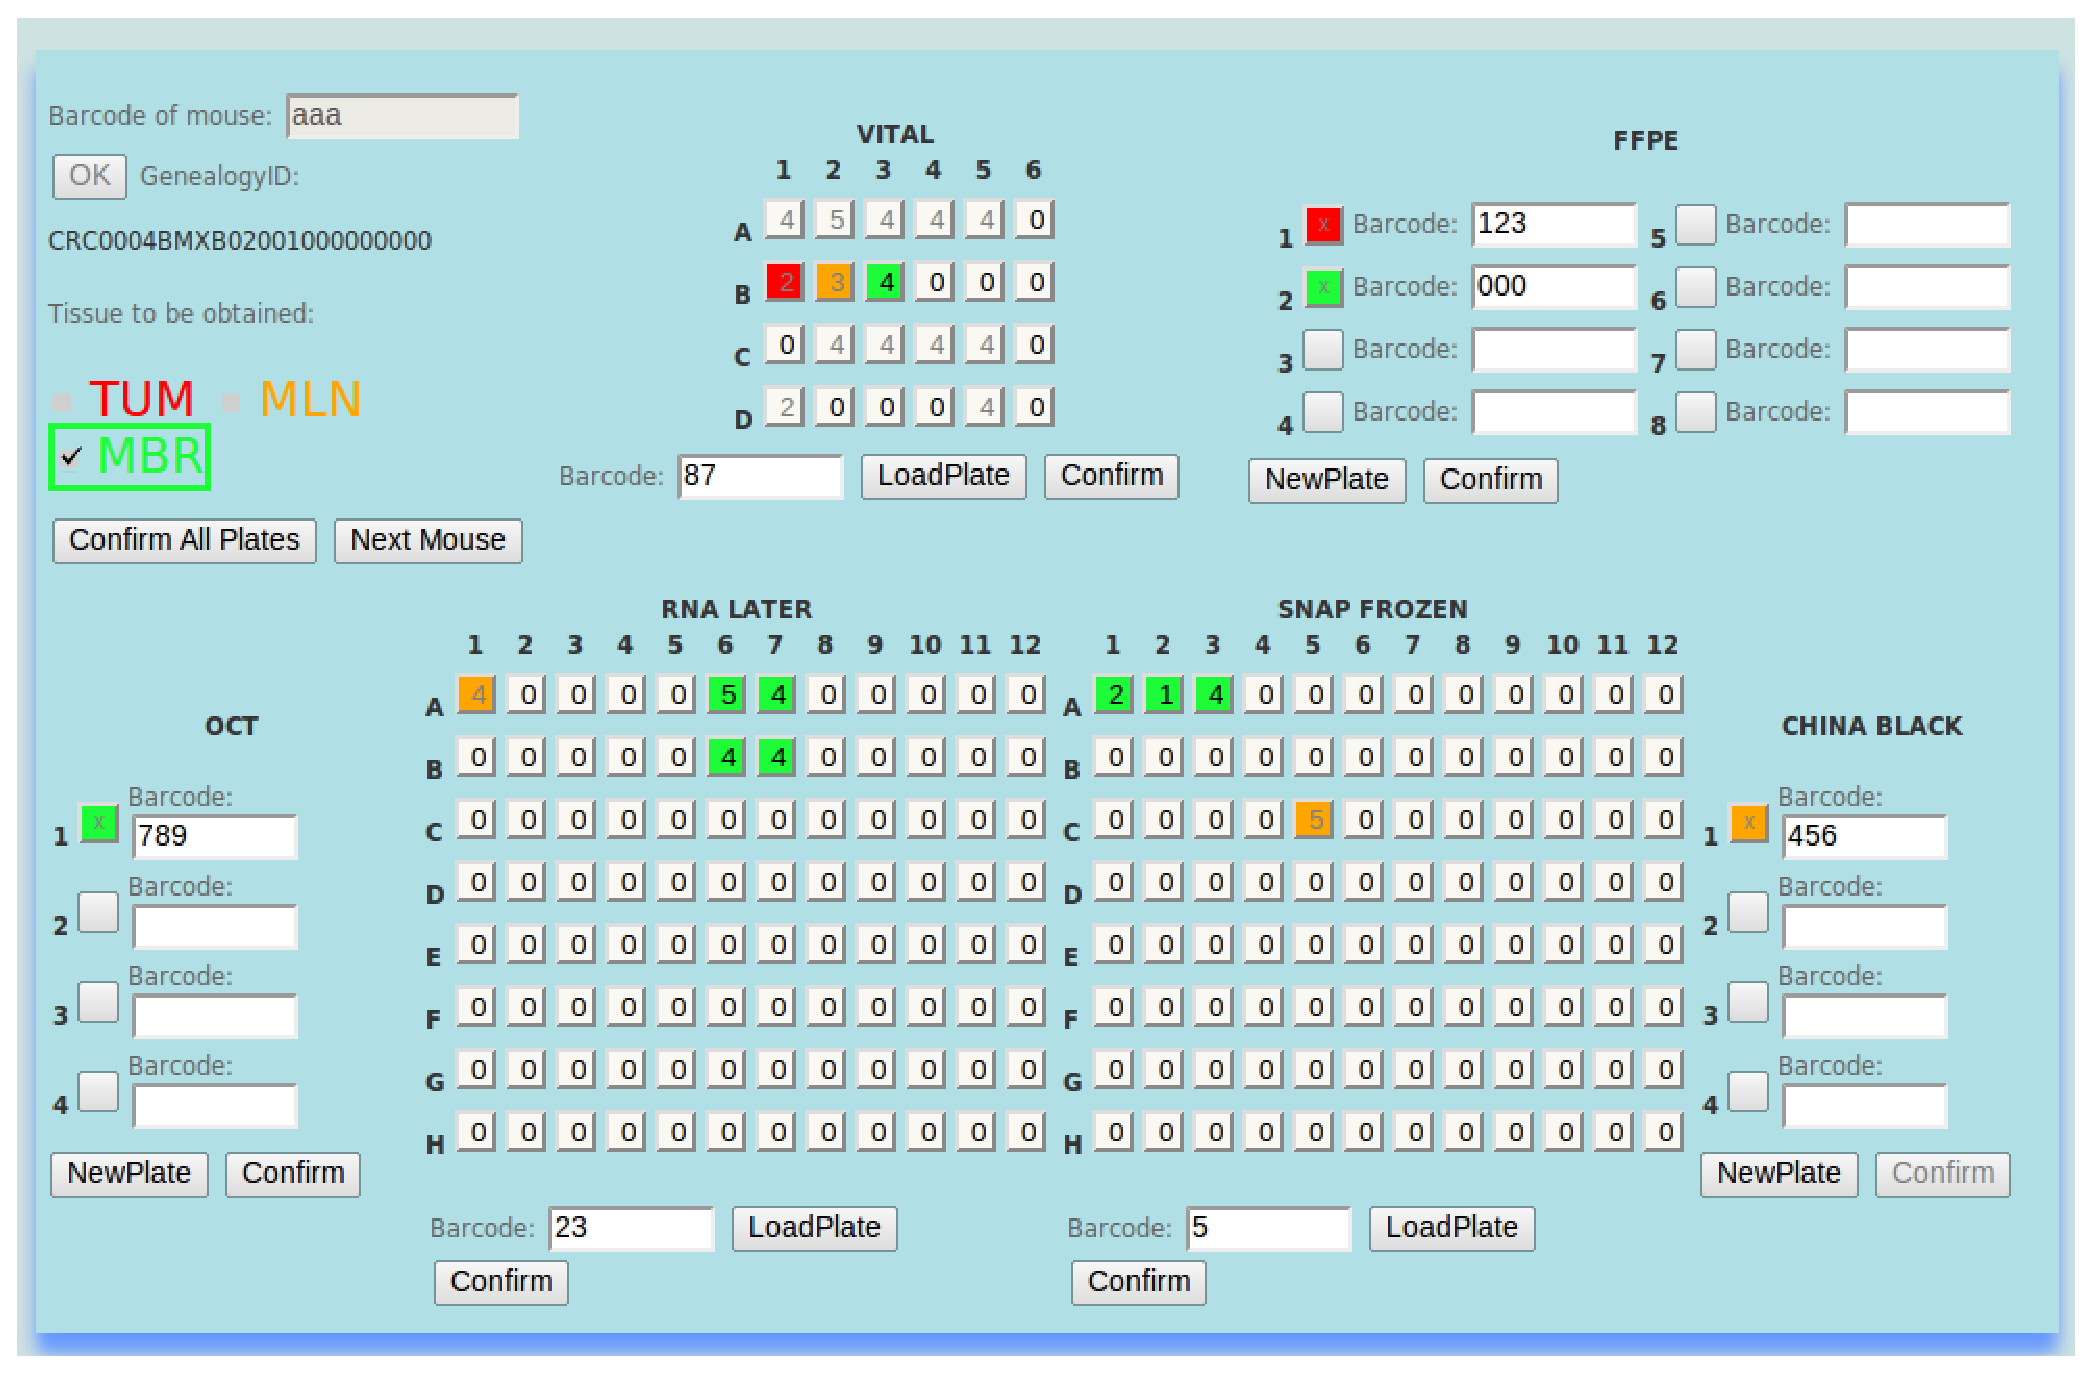
\includegraphics[width=1.0\textwidth]{./Figure/explantForm}
\end{center}
\caption{Struttura della pagina per collezionare i vari tessuti\label{fig:explForm}}
\end{figure}\newpage

L'operatore, per inserire le aliquote in queste tabelle, procede inserendo il barcode dello xenopaziente da espiantare. Successivamente, carica i dati delle piastre sulle quali vuole lavorare, inviandone cos\`i il barcode alla BioBanca. Dopodich\`e, inserisce i singoli tessuti nelle varie provette, a seconda del tipo di conservazione. In caso di errore, si pu\`o rimediare attraverso un'apposita lista, nella quale sono inserite le ultime operazioni effettuate. 

Una volta espiantati tutti i topi precedentemente selezionati, si procede con il salvataggio, articolato in pi\`u fasi. Si inviano i dati di tutte le aliquote create nella serie alla BioBanca, la quale tenta di salvarle nel proprio database. All'applicazione \Xeno\ arriva il responso sull'esito della transazione. In caso positivo, XMS avvia a sua volta il salvataggio dei dati. L'esito di questa operazione \`e notificata alla BioBanca, che, in caso negativo, effettua il rollback sulle informazioni precedentemente salvate. Infine, a seconda degli esiti delle precedenti operazioni, si visualizza il report dei dati creati o un messaggio d'errore. Questo flusso logico di dati \`e descritto in Figura~\ref{fig:flussoExpl}, mentre in Figura~\ref{fig:SDexpl} si pu\`o osservare il diagramma delle sequenze di questa interfaccia.


\begin{figure}[h]
\begin{center}
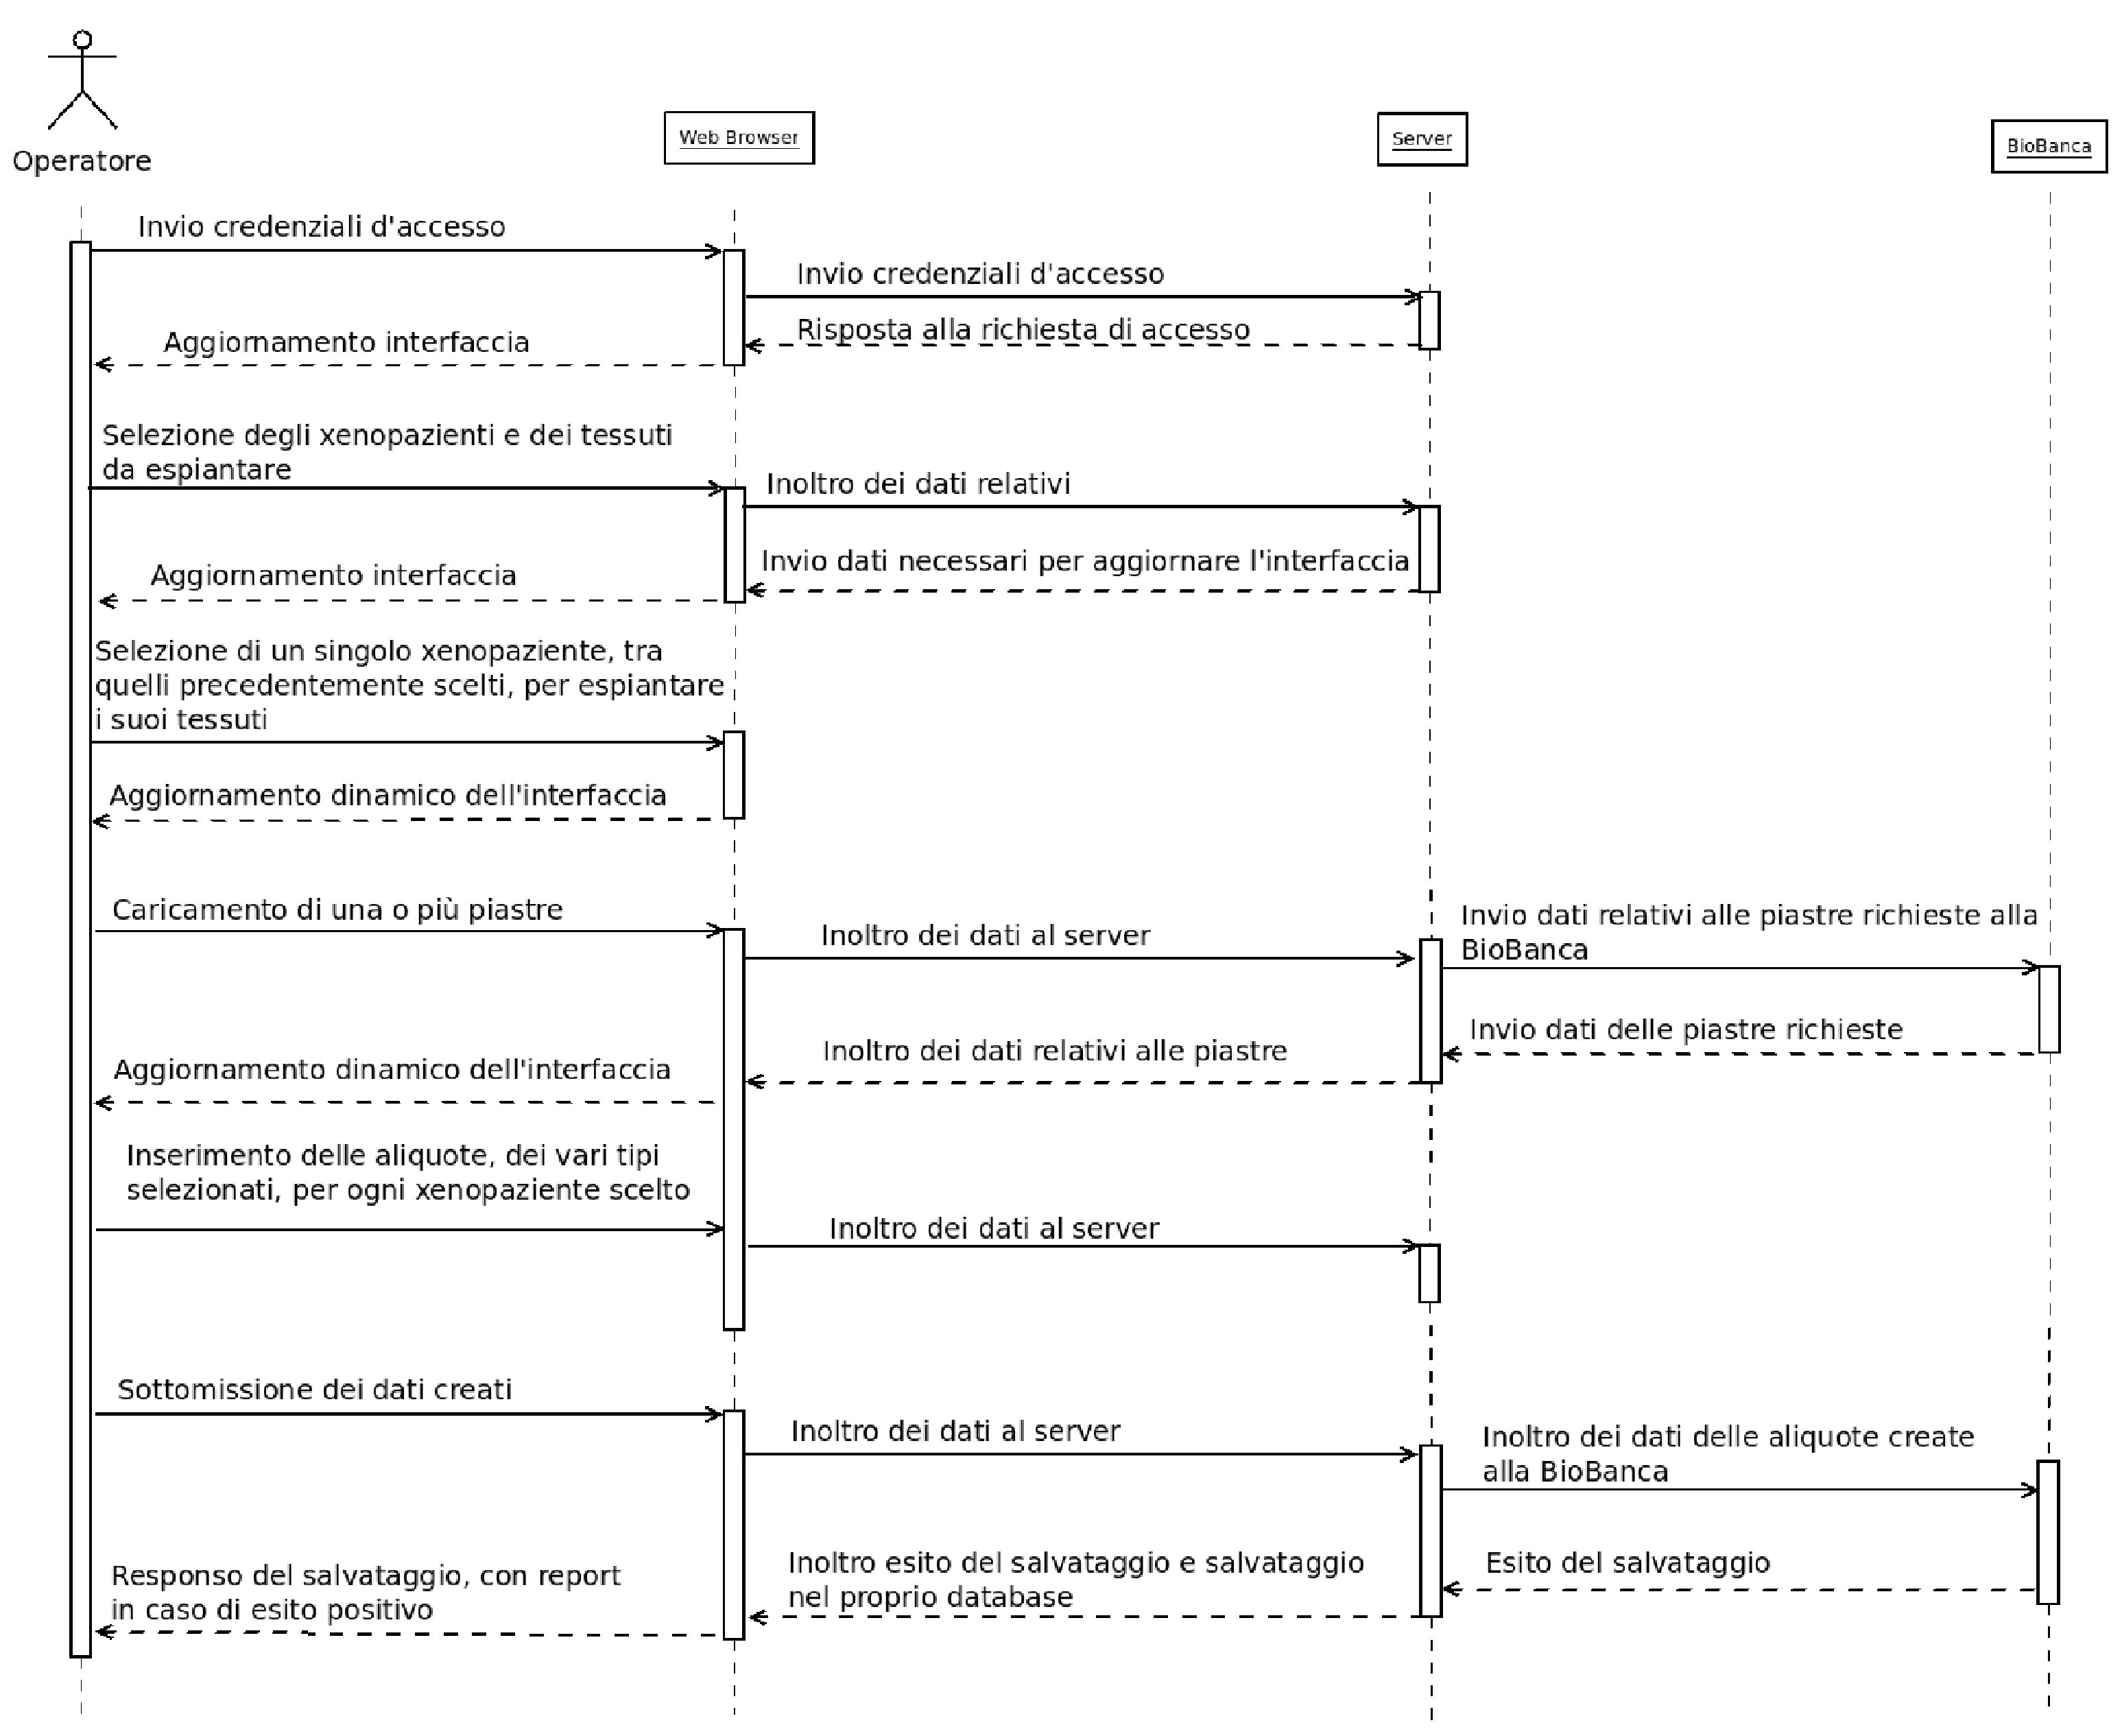
\includegraphics[width=0.9\textwidth]{./Figure/SDexplants}
\end{center}
\caption{Diagramma delle sequenze relativo agli espianti\label{fig:SDexpl}}
\end{figure}

\begin{figure}[h]
\begin{center}
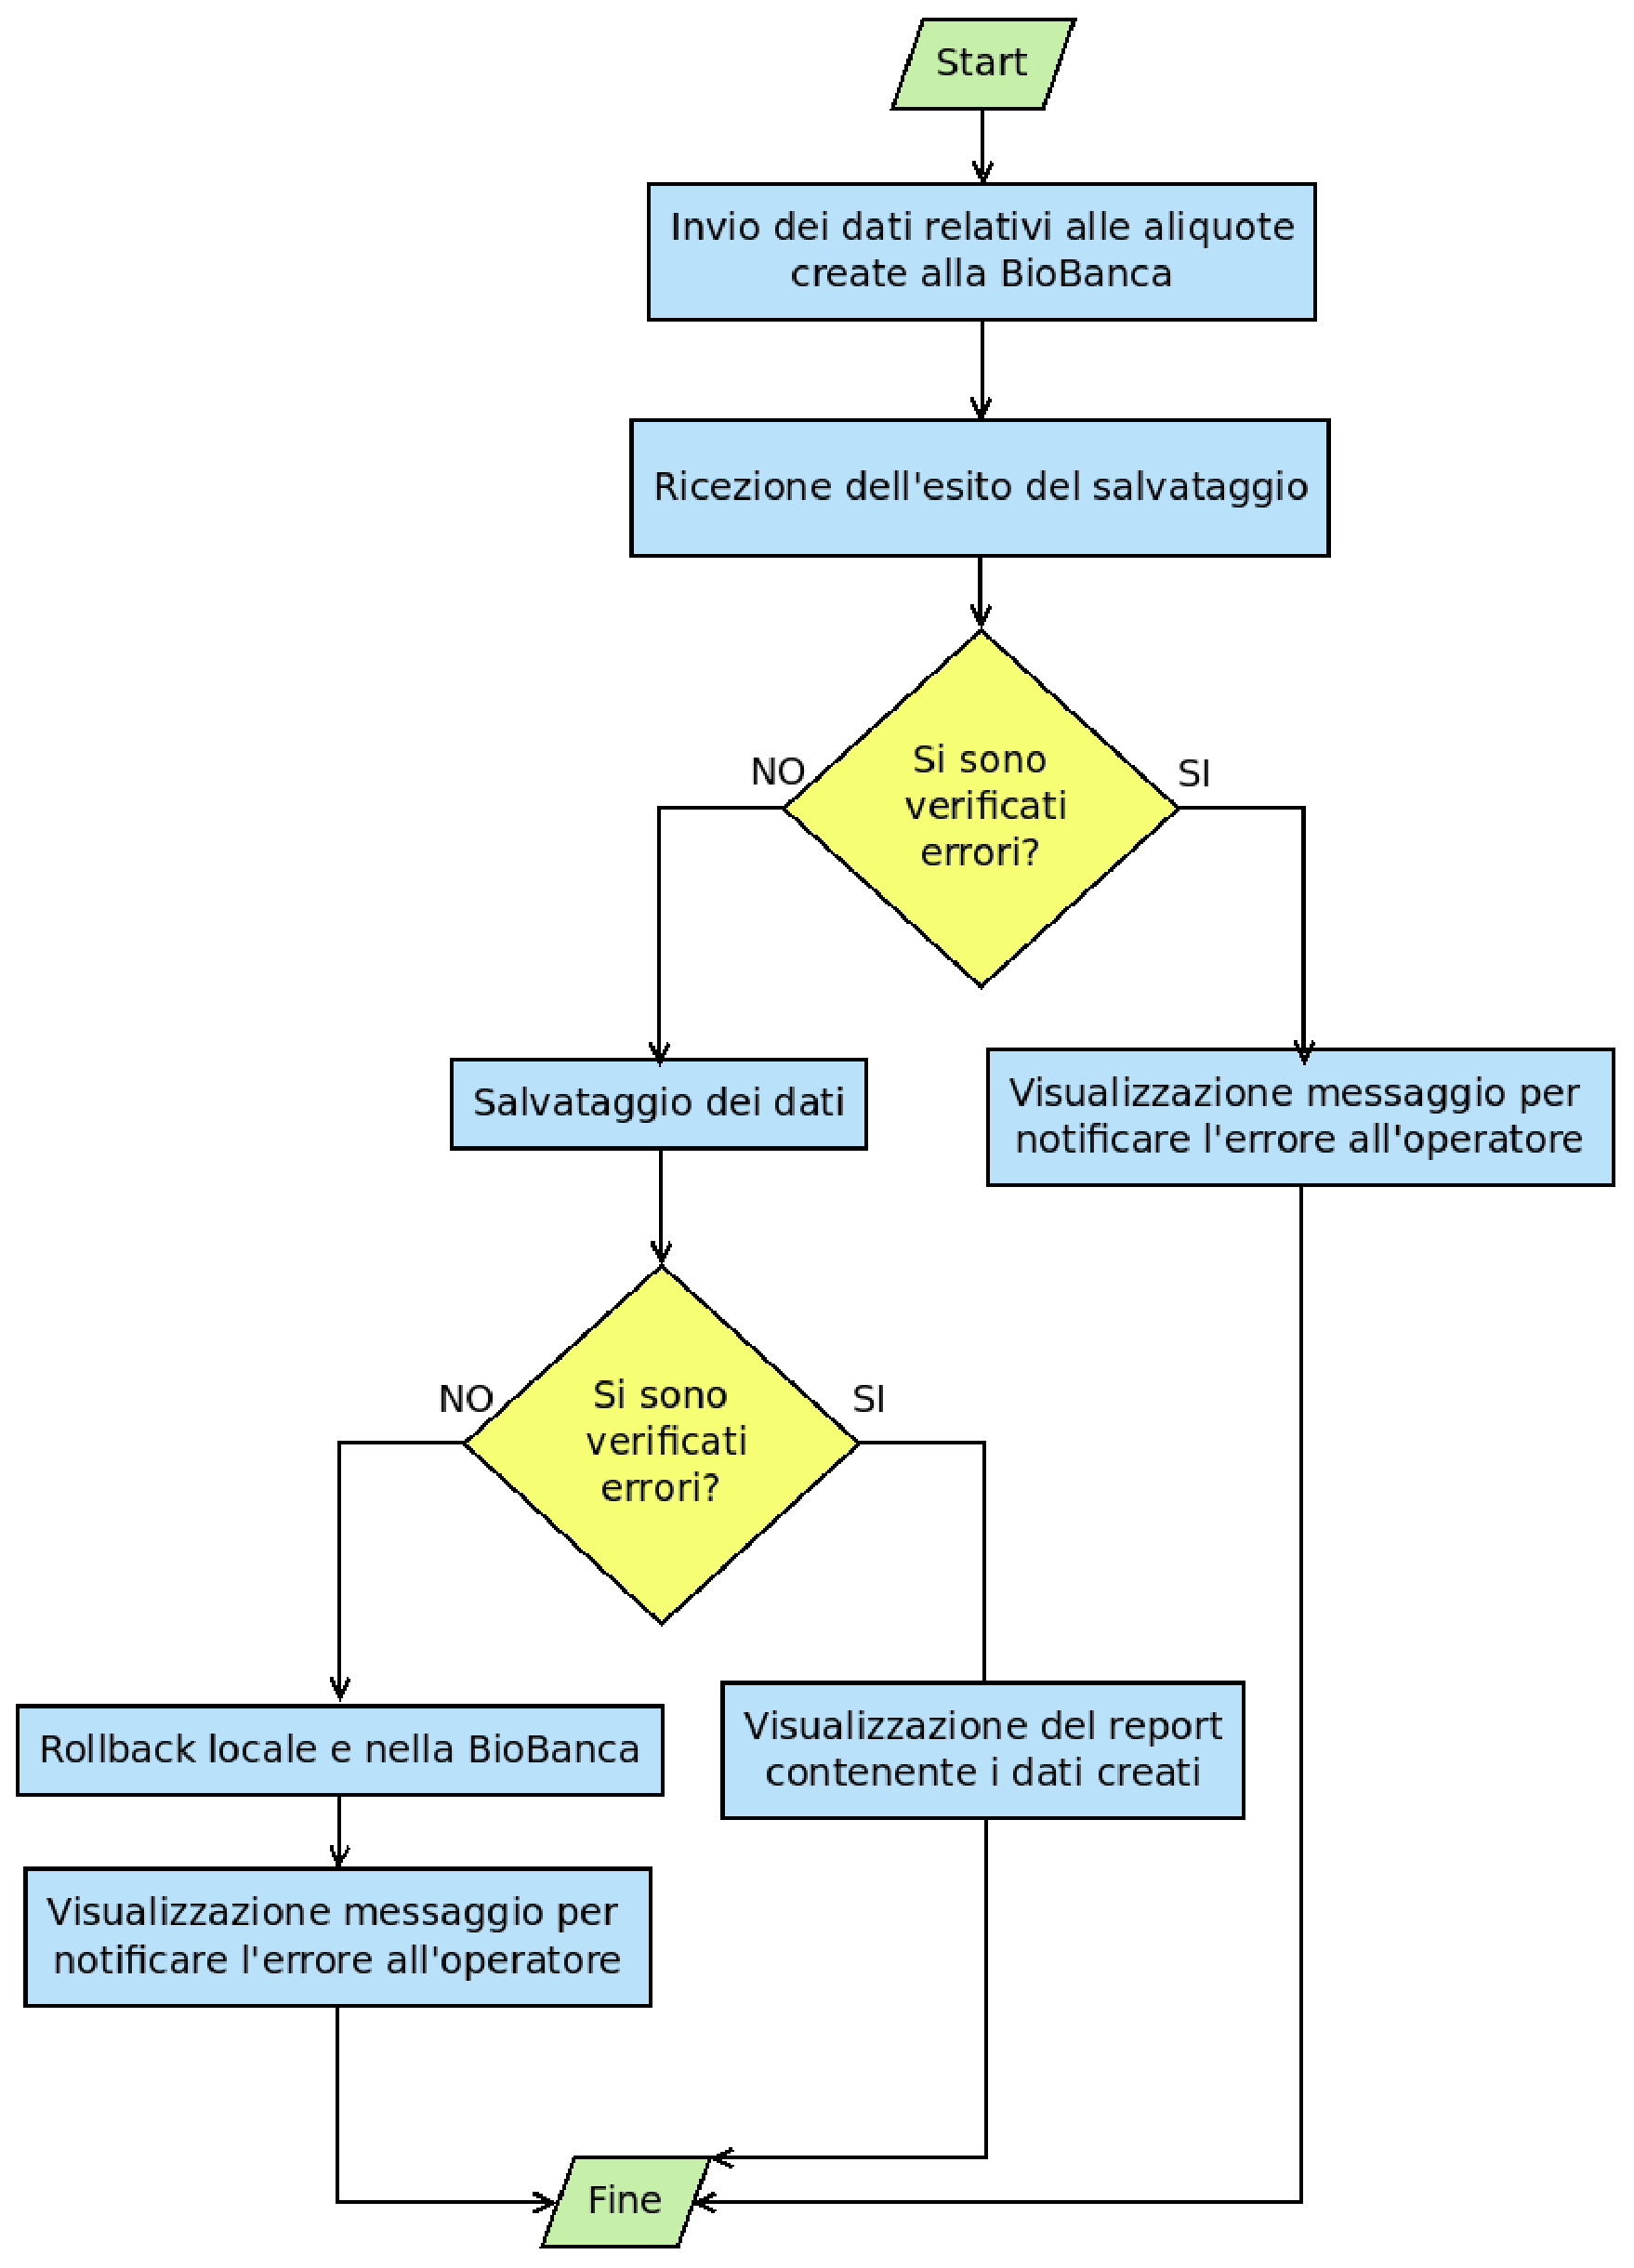
\includegraphics[width=0.8\textwidth]{./Figure/flussoExplants}
\end{center}
\caption{Diagramma di flusso delle comunicazione con la BioBanca\label{fig:flussoExpl}}
\end{figure}


\chapter{Conclusioni}\label{chap:xenoconcl}

\Xeno\ ha come scopo principale quello di risolvere e gestire correttamente i problemi derivanti dalla sperimentazione sugli xenopazienti. \`E quindi necessario poter gestire tutte le operazioni inerenti al ciclo di vita dei topi, tra le quali sono presenti la gestione degli impianti/espianti, le misurazioni e il caricamento di nuovi individui nel sistema. Le operazioni appena descritte devono essere gestite rispettando i numerosi vincoli relazionali presenti tra i vari dati da amministrare e creare. Tutto ci\`o \`e stato risolto creando un apposito database relazionale, modellandolo in modo tale da riuscire a soddisfare al meglio le specifiche richieste dell'istituto.

L'applicazione XMS \`e stata implementata attraverso una Web Application, la quale soddisfa al meglio i precisi requisiti dell'IRCC di Candiolo. Si \`e scelta questa soluzione per poter fornire un servizio facilmente accessibile, dove gli unici requisti sono una connessione alla rete ed un Web browser. L'applicazione \`e stata sviluppata secondo il paradigma Model View Controller, mediante l'utilizzo di Django, un framework scritto in Python per la creazione di Web Application. La scelta del design pattern MVC consente di conferire al sistema una struttura modulare, permettendo cos\`i di poter intervenire in maniera puntuale e minimale in caso di modifiche dell'applicazione. Il sistema \`e stato progettato in modo tale da ottenere una distribuzione della business logic tra client e server, demandando alcune operazioni direttamente al browser dell'operatore. 

XMS offre una serie di funzionalit\`a legate allo studio e alla ricerca sugli xenopazienti. Per gestire la colonia di topi, \`e possibile inserire nuovi individui nel sistema e, eventualmente, aggiornarne lo status attuale. \`E anche possibile amministrare le operazioni di impianto, mediante le quali si immettono delle aliquote di tessuto all'interno degli xenopazienti. Inoltre, \`e necessario fornire all'utente la possibilit\`a di misurare la crescita della massa tumorale, in risposta a determinati trattamenti assegnati ai vari topi. Infine, si \`e implementata la gestione degli espianti, operazioni mediante le quali si asportono dagli xenopazienti le masse tumorali precedentemente impiantate. Questo funzionalit\`a sono utilizzabili dall'utente tramite apposite interfacce. Ognuna di queste \`e stata costruita in modo da permettere una veloce interazione con l'operatore. Inoltre, per consentire una maggiore integrazione con i sistemi in uso presso l'IRCC, si \`e gestita la compatibilit\`a con i lettori di chip RFID e di codici a barre. 

Per svolgere con maggiore efficienza i suoi compiti, \Xeno\ deve poter cooperare con gli altri moduli del LAS. In particolare, XMS accede ai dati relativi alle aliquote presenti nel sistema, creando cos\`i un flusso di comunicazione con la BioBanca. Inoltre, XMS, deve essere in grado di fornire determinate informazioni, quando richieste, alle altre applicazioni, rendendo possibili elaborazioni pi\`u dettagliate ed approfondite. Per supportare tali funzionalit\`a, \`e stata implementata una serie di Application Programming Interface (API), utili, ad esempio, per la gestione della business logic all'interno di XMS. Infatti, alcune API sono state utilizzate per effettuare controlli nel database durante l'immissione di dati da parte dell'operatore, prelevando i dati degli xenopazienti coinvolti nelle varie operazioni, ed evitando cos\`i l'inserimento di dati duplicati. Inoltre, le API risultano fondamentali per le interazioni con gli altri moduli del LAS, fornendo i dati da essi richiesti. 

Come visto nel Capitolo~\ref{chap:xenocase}, XMS offre un ambiente di lavoro in grado di simulare il laboratorio, dove ogni giorno operano i ricercatori. Questa simulazione \`e stata ottenuta soprattutto nelle interfacce relative alle operazioni di impianti ed espianti, creando schermate agevoli per gli operatori, i quali ritrovano una corrispondenza tra l'applicazione e il mondo reale.

\section{Sviluppi futuri}

Durante la progettazione e lo sviluppo di questa Web Application, si sono individuate varie possiblit\`a di ampliamento. Ogni singola miglioria contribuir\`a a perfezionare le prestazioni e i servizi offerti dal sistema.

I trattamenti sugli xenopazienti rappresentano una funzione gestita da \Xeno. Per offrire una maggior assistenza agli operatori, una possibilit\`a consiste nell'implementare un sistema di \textbf{e-mail alerting}, in modo tale da poter amministrare con maggior efficenza l'interruzione programmata dei vari trattamenti. Con questa funzione ulteriore, gli utenti (e i loro supervisori) riceverebbero una notifica nella loro casella di posta elettronica nel momento in cui sia imminente la fine di un trattamento precedentemente avviato.

Una nuova interfaccia che potrebbe essere implementata avrebbe il compito di effettaure il \textbf{check delle misure}. Si tratta di una serie di funzionalit\`a atte a verificare la bont\`a delle operazioni svolte dai vari utenti. Sar\`a accessibile solo all'amministratore del sistema, il quale potr\`a visionare tutte le azioni non ancora validate portate a termine dagli operatori. Successivamente, potr\`a scegliere se confermare, annullare o modificare le scelte prese dagli altri utenti. In questo modo, si porr\`a sulle operazioni svolte un controllo che esula dalle pure verifiche informatiche, ma che va anche ad analizzare la validit\`a scientifica dei dati.

Infine, un ultimo lavoro molto importante, sar\`a il recupero dei dati storici dell'IRCC di Candiolo, in modo tale da poter inserire nel database anche le informazioni relative agli xenopazienti degli anni passati. Questo permettar\`a a \Xeno\ di avere al suo interno un consistente storico di dati, potenziando cos\`i fin da subito la sua utilit\`a.

\chapter{Tabelle del database}\label{chap:xenotable}

Gli attributi contrassegnati con '*' sono da considerarsi nullabili; quelli scritti in grassetto rappresentano la chiave primaria e quelli in italico sono le chiave esterne. Sono stati considerati nullabili vari attributi della tabella Mice in quanto tali dati potrebbero non essere presenti nello storico dei topi. Le tabelle contenenti la parola '\_has\_' al loro interno sono utilizzate per modellare le relazioni molti a molti tra le tabelle ad esse collegate. 

\section{Xenopazienti}

\textbf{Tabella Mice}

\begin{longtable}{|l|l|p{4.4cm}|}
\hline
\textbf{Nome campo} &	\textbf{Tipo} &	\textbf{Descrizione}\\ \hline
\textbf{id} &	BIGINT &	Identifcativo del topo\\ \hline
\textit{idMouseStrain}* &	BIGINT &	Identifcativo della razza del topo\\ \hline
\textit{idStatus} &	INT &	Identificativo dello status attuale del topo\\ \hline
barcode* &	VARCHAR(15) &	Codice del chip assegnato al topo\\ \hline
availableDate* &	DATE &	Data a partire dalla quale il topo \`e pronto per la sperimentazione\\ \hline
deathDate* &	DATE &	Data di morte del topo\\ \hline
\textit{id\_genalogy}* &	VARCHAR(15) &	Genealogia dell'impianto nel topo\\ \hline
\textit{id\_cancer\_research\_group} &	INT &	Gruppo di ricerca a cui \`e assegnato il topo.\\ \hline
\textit{id\_source}&	INT &	Chi ha fornito il topo al centro di ricerca.\\ \hline
gender &	ENUM('m','f') &	Sesso del topo.\\ \hline
birth\_date &	DATE &	Data presunta di nascita del topo.\\ \hline
notes* &	VARCHAR(150) &	Eventuali commenti (ad esempio, in caso di morte non naturale)\\ \hline
\caption{Tabella Mice}
\end{longtable}

\textbf{Tabella MouseStrain}

\begin{longtable}{|l|l|p{5.5cm}|}
\hline
\textbf{Nome campo} &	\textbf{Tipo} &	\textbf{Descrizione}\\ \hline
\textbf{id} &	INT &	Identificativo della razza del topo\\ \hline
mouse\_type\_name &	VARCHAR(50) &	Nome della razza\\ \hline
description* &	VARCHAR(150) &	Campo per eventuali descrizioni aggiuntive\\ \hline
linkToDoc* &	VARCHAR(150) & URL riferente alla documentazione ufficiale della razza\\ \hline
\caption{Tabella MouseStrain}
\end{longtable}

\textbf{Tabella Source}

\begin{longtable}{|l|l|p{5.5cm}|}
\hline
\textbf{Nome campo} &	\textbf{Tipo} &	\textbf{Descrizione}\\ \hline
\textbf{id} &	INT &	Identificativo del fornitore di xenopazienti\\ \hline
name &	VARCHAR(45) &	Nome del fornitore\\ \hline
description* &	VARCHAR(45) &	Campo per eventuali descrizioni aggiuntive\\ \hline
\caption{Tabella Source}
\end{longtable}


\textbf{Tabella Status}

\begin{longtable}{|l|l|p{6.2cm}|}
\hline
\textbf{Nome campo} &	\textbf{Tipo} &	\textbf{Descrizione}\\ \hline
\textbf{id} &	INT &	Identificativo dello stato attuale del topo\\ \hline
name &	VARCHAR(50) &	Nome dello stato attuale del topo\\ \hline
description* &	VARCHAR(150) &	Campo per eventuali descrizioni aggiuntive\\ \hline
default &	BOOLEAN &	Stato di default per i topi inseriti dalla schermata Mice Loading\\ \hline
\caption{Tabella Status}
\end{longtable}

\textbf{Tabella ChangeStatus}

\begin{longtable}{|l|l|p{5.5cm}|}
\hline
\textbf{Nome campo} &	\textbf{Tipo} &	\textbf{Descrizione}\\ \hline
\textbf{id} & INT & Chiave della tabella\\ \hline
\textit{from\_status} & INT & Status di partenza\\ \hline
\textit{to\_status} & INT & Status di arrivo\\ \hline
\caption{Tabella ChangeStatus}
\end{longtable}


\textbf{Tabella StatusInfo}

\begin{longtable}{|l|l|p{7.0cm}|}
\hline
\textbf{Nome campo} &	\textbf{Tipo} &	\textbf{Descrizione}\\ \hline
\textbf{id} &	INT &	Identificativo delle informazioni aggiuntive sullo status\\ \hline
description &	VARCHAR(45) &	Descrizione dell'informazione aggiuntiva\\ \hline
\caption{Tabella StatusInfo}
\end{longtable}

\textbf{Tabella Status\_info\_has\_status}

\begin{longtable}{|l|l|p{8.0cm}|}
\hline
\textbf{Nome campo} &	\textbf{Tipo} &	\textbf{Descrizione}\\ \hline
\textbf{id} &	INT &	Identificativo\\ \hline
id\_status &	INT &	Identificativo dello status a cui ci si riferisce\\ \hline
id\_info &	INT &	Identificativo dell'informazione aggiuntiva associata allo status.\\ \hline
\caption{Tabella Status\_info\_has\_status}
\end{longtable}

\section{Impianti - Espianti}

\textbf{Tabella Aliquots}

\begin{longtable}{|l|l|p{5.5cm}|}
\hline
\textbf{Nome campo} &	\textbf{Tipo} &	\textbf{Descrizione}\\ \hline
\textbf{id} &	BIGINT &	Identifcativo dell'aliquota\\ \hline
\textit{TypeOfTisue} &	INT &	Identficativo della tabella contenente i diversi tipi di tessuto dell'aliquota\\ \hline
\textbf{idExplant*} &	BIGINT &	Id dell'eventuale espianto da cui viene prodotta\\ \hline
id\_genealogy & VARCHAR(15) & Identificativo della genealogia a cui appartiene l'aliquota\\ \hline
\caption{Tabella Aliquots}
\end{longtable}

\textbf{Tabella TissueType}

\begin{longtable}{|l|l|p{5.5cm}|}
\hline
\textbf{Nome campo} &	\textbf{Tipo} &	\textbf{Descrizione}\\ \hline
\textbf{id} &	INT &	Identificativo del tipo di tessuto\\ \hline
\textit{abbreviation} &	VARCHAR(3) &	Abbreviazione univoca, in 3 lettere, del tipo di tessuto\\ \hline
\textit{name} &	VARCHAR(45) &	Nome completo del tipo di tessuto\\ \hline
notes* &	VARCHAR(150) &	Eventuali note\\ \hline
\caption{Tabella TissueType}
\end{longtable}

\textbf{Tabella Series}

\begin{longtable}{|l|l|p{5.5cm}|}
\hline
\textbf{Nome campo} &	\textbf{Tipo} &	\textbf{Descrizione}\\ \hline
\textbf{id} &	BIGINT &	Identificativo della serie\\ \hline
\textit{idOperator} &	BIGINT &	Identificativo dell'operatore\\ \hline
\textit{idScope} &	INT &	Identficativo della tabella contenente i vari scopi possibili\\ \hline
\textit{idTypeOfSerie} &	INT &	Identficativo della tabella contenente le varie operazioni possibili\\ \hline
date &	DATE &	Data della serie\\ \hline
notes* &	VARCHAR(150) &	Eventuali commenti\\ \hline
\caption{Tabella Series}
\end{longtable}

\textbf{Tabella Type\_of\_serie}

\begin{longtable}{|l|l|p{5.5cm}|}
\hline
\textbf{Nome campo} &	\textbf{Tipo} &	\textbf{Descrizione}\\ \hline
\textbf{id} &	INT &	Identificativo del tipo della serie\\ \hline
\textit{description} &	VARCHAR(45) &	Breve descrizione della serie \\ \hline
\caption{Tabella Type\_of\_serie}
\end{longtable}

\textbf{Tabella ImplantDetails}

\begin{longtable}{|l|l|p{7.0cm}|}
\hline
\textbf{Nome campo} &	\textbf{Tipo} &	\textbf{Descrizione}\\ \hline
\textbf{id} &	BIGINT &	Identificavitvo dell'impianto\\ \hline
\textit{idMouse} &	BIGINT &	Identificativo del topo\\ \hline
\textit{idSeries} &	BIGINT &	Identificativo della serie di impianti\\ \hline
\textit{idAliquot} &	BIGINT &	Identificativo dell'aliquota usata\\ \hline
BadQualityFlag &	BOOLEAN &	Flag per indicare la riuscita o meno dell'impianto (ad esempio, se si rovina l'aliquota mentre la si impianta)\\ \hline
site & INT & Riferimento alla tabella Site, per individuare l'impianto nel topo\\ \hline
\caption{Tabella ImplantDetails}
\end{longtable}

\subsubsection{Tabella Site}

\begin{longtable}{|l|l|p{5.5cm}|}
\hline
\textbf{Nome campo} &	\textbf{Tipo} &	\textbf{Descrizione}\\ \hline
\textbf{id} &	BIGINT &	Identificavitvo del sito dell'impianto\\ \hline
name &	VARCHAR(2) & Abbreviazione del nome del sito su due lettere\\ \hline
longName &	VARCHAR(50) & Nome del sito\\ \hline
\caption{Tabella Site}
\end{longtable}

\textbf{Tabella ExplantDetails}

\begin{longtable}{|l|l|p{5.5cm}|}
\hline
\textbf{Nome campo} &	\textbf{Tipo} &	\textbf{Descrizione}\\ \hline
\textbf{id} &	BIGINT &	Identificativo dell'espianto\\ \hline
\textit{idSeries} &	BIGINT &	Identificativo della serie di espianti\\ \hline
\textit{idMouse} &	BIGINT &	Identificativo del topo\\ \hline
\caption{Tabella ExplantsDetails}
\end{longtable}

\textbf{Tabella Programmed\_explant}

\begin{longtable}{|l|l|p{5.5cm}|}
\hline
\textbf{Nome campo} &	\textbf{Tipo} &	\textbf{Descrizione}\\ \hline
\textbf{id} &	INT &	Identificativo dell'espianto programmato\\ \hline
\textit{idScope} &	INT &	Identificativo dello scopo dell'espianto\\ \hline
\textit{idMouse} &	BIGINT &	Identificativo dello xenopaziente su cui \`e stato programmato l'espianto\\ \hline
done &	BOOLEAN &	Flag per indicare il completamento dell'espianto programmato\\ \hline
\caption{Tabella Programmed\_explant}
\end{longtable}

\textbf{Tabella ScopeDetails}

\begin{longtable}{|l|l|p{5.5cm}|}
\hline
\textbf{Nome campo} &	\textbf{Tipo} &	\textbf{Descrizione}\\ \hline
\textbf{idScope} &	INT &	Identificativo dello scopo\\ \hline
description &	VARCHAR(250) &	Descrizione dello scopo\\ \hline
\caption{Tabella ScopeDetails}
\end{longtable}

\section{Operatori}

\subsubsection{Tabella auth\_user}

\begin{longtable}{|l|l|p{6.5cm}|}
\hline
\textbf{Nome campo} &	\textbf{Tipo} &	\textbf{Descrizione}\\ \hline
\textbf{id} &	BIGINT &	Identificativo dell'operatore\\ \hline
username &	VARCHAR(30) &	Username dell'operatore\\ \hline
first\_name &	VARCHAR(20) &	Nome dell'operatore\\ \hline
last\_name &	VARCHAR(45) &	Cognome dell'operatore\\ \hline
email &	VARCHAR(30) &	Contatto dell'operatore\\ \hline
password &	VARCHAR(128) &	Password dell'operatore (salvata dopo essere stata sottoposta ad una funzione di hash)\\ \hline
is\_staff & BOOLEAN & Flag per indicare se l'utente pu\`o accedere all'interfaccia di admin\\ \hline
is\_active & BOOLEAN & Flag per indicare se l'account \`e in uso o meno; l'uso di questo flag pu\`o sostituire la cancellazione fisica dell'account nel caso in cui lo si voglia eliminare dal sistema\\ \hline
is\_superuser & BOOLEAN & Flag per indicare se l'utente \`e l'amministratore del sistema\\ \hline
last\_login & DATATIME & Data dell'ultimo login di questo operatore\\ \hline
date\_joined & DATETIME & Data in cui \`e stato creato l'account\\ \hline
\caption{Tabella auth\_user}
\end{longtable}

\subsubsection{Tabella XenoUsers }

\begin{longtable}{|l|l|p{6.5cm}|}
\hline
\textbf{Nome campo} &	\textbf{Tipo} &	\textbf{Descrizione}\\ \hline
\textit{\textbf{user\_ptr\_id}}  &	INT &	Identificativo dell'utente (operatore) a cui si riferiscono le informazioni aggiuntive.\\ \hline
\textit{id\_supervisor*} &	 INT &	Identificativo dell'eventuale supervisore\\ \hline
\textit{id\_institution} &	INT &	Identificativo dell'istituto di appartenenza.\\ \hline
\textit{id\_cancer\_research\_group} &	INT &	Identificativo del gruppo di ricerca di appartenenza.\\ \hline
\caption{Tabella XenoUsers}
\end{longtable}

\subsubsection{Tabella cancer\_research\_group}

\begin{longtable}{|l|l|p{5.5cm}|}
\hline
\textbf{Nome campo} &	\textbf{Tipo} &	\textbf{Descrizione}\\ \hline
\textbf{idCancerResearchGroup} &	INT &	Identificativo del gruppo di ricerca\\ \hline
name &	VARCHAR(255) &	Nome del gruppo di ricerca\\ \hline
\caption{Tabella cancer\_research\_group}
\end{longtable}

\subsubsection{Tabella institution}

\begin{longtable}{|l|l|p{5.5cm}|}
\hline
\textbf{Nome campo} &	\textbf{Tipo} &	\textbf{Descrizione}\\ \hline
\textbf{idInstitution} &	INT &	Identificativo dell'istituzione/ente\\ \hline
name &	VARCHAR(255) &	Nome dell'istituzione/ente\\ \hline
\caption{Tabella Institution}
\end{longtable}

\section{Gestione misurazioni}

\subsubsection{Tabella MeasurementSeries}

\begin{longtable}{|l|l|p{7.5cm}|}
\hline
\textbf{Nome campo} &	\textbf{Tipo} &	\textbf{Descrizione}\\ \hline
\textbf{id} &	BIGINT &	Identificativo della serie di misure\\ \hline
\textit{idOperator} &	BIGINT &	Identificativo dell'operatore che ha effettuato la misura\\ \hline
date &	DATE &	Data della misura\\ \hline
\textit{id\_type*} & INT & Indica con quale tipologia di misurazione sono state effettuate le misure della serie\\ \hline
\caption{Tabella MeasurementSeries}
\end{longtable}

\subsubsection{Tabella QualitativeMeasure}

\begin{longtable}{|l|l|p{6.0cm}|}
\hline
\textbf{Nome campo} &	\textbf{Tipo} &	\textbf{Descrizione}\\ \hline
\textbf{id} &	INT & Identificativo della misura qualitativa\\ \hline
\textit{id\_value} & INT &	Valore della misurazione\\ \hline
\textit{id\_series} & INT &	Serie di appartenenza della misura\\ \hline
\textit{id\_mouse} & INT &	Topo su cui \`e stata effettuata la misura\\ \hline
notes* &	VARCHAR(255) & Eventuali note sulla misurazione\\ \hline
\caption{Tabella QuantitativeMeasure}
\end{longtable}

\subsubsection{Tabella Qualitative\_values}

\begin{longtable}{|l|l|p{6.5cm}|}
\hline
\textbf{Nome campo} &	\textbf{Tipo} &	\textbf{Descrizione}\\ \hline
\textbf{id} &	INT &	Identificativo del valore qualitativo\\ \hline
value &	VARCHAR(45) &	Uno dei valori ammissibili per la misura qualitativa (es. 'Large', 'None',..)\\ \hline
description* &	VARCHAR(45) &	Eventuale descrizione.\\ \hline
\caption{Tabella Qualitative\_values}
\end{longtable}

\subsubsection{Tabella QuantitativeMeasure}

\begin{longtable}{|l|l|p{5.5cm}|}
\hline
\textbf{Nome campo} &	\textbf{Tipo} &	\textbf{Descrizione}\\ \hline
\textbf{id} &	INT &	Identificativo del valore quantitativo\\ \hline
x\_measurement &	DOUBLE &	Valore X ottenuto dalla misurazione\\ \hline
y\_measurement &	DOUBLE &	Valore Y ottenuto dalla misurazione\\ \hline
volume &	DOUBLE &	Volume ottenuto dopo un calcolo su X e Y.\\ \hline
\textit{id\_series} & INT &	Serie di appartenenza della misura\\ \hline
\textit{id\_mouse} & INT &	Topo su cui \`e stata effettuata la misura\\ \hline
notes* &	VARCHAR(255) & Eventuali note sulla misurazione\\ \hline
\caption{Tabella QuantitativeMeasure}
\end{longtable}

\subsubsection{Tabella TypeOfMeasure}

\begin{longtable}{|l|l|p{6.5cm}|}
\hline
\textbf{Nome campo} &	\textbf{Tipo} &	\textbf{Descrizione}\\ \hline
\textbf{id} &	BIGINT &	Identificativo del tipo di misura\\ \hline
name &	VARCHAR(99) &	Nome della tipologia di misura (attualmente, assume valori 'qualitative' o 'quantitative'.\\ \hline
\caption{Tabella TypeOfMeasure}
\end{longtable}

\subsection{Gestione dei trattamenti}

\subsubsection{Tabella Treatments}

\begin{longtable}{|l|l|p{5.5cm}|}
\hline
\textbf{Nome campo} & \textbf{Tipo} & \textbf{Descrizione}\\ \hline
\textbf{id} & INT & Identificativo del trattamento\\ \hline
name	 & INT & 	Nome del trattamento\\ \hline
description & INT & Breve descrizione del trattamento\\ \hline
duration	& INT & Durata prevista (in giorni o ore) del trattamento\\ \hline
type\_of\_time & ENUM(hours, days) & Questo campo serve a definire se la durata \`e specificata in ore o giorni\\ \hline
forces\_explant & BOOLEAN & Questo campo assume valore True o False a seconda del fatto che il trattamento sia acuto o meno.\\ \hline
\caption{Tabella Treatments}
\end{longtable}

\subsubsection{Tabella Detail\_treatments}

\begin{longtable}{|l|l|p{6.5cm}|}
\hline
\textbf{Nome campo} &	\textbf{Tipo} &	\textbf{Descrizione}\\ \hline
\textbf{id}	&	INT	&	Identificativo (inserito per compatibilit\`a con Django)\\ \hline
\textit{id\_via}	&	INT	&	Identifica la via di somministrazione\\ \hline
\textit{treatments\_id} &		INT	&	Identifica il trattamento di cui si stanno specificando i vari step\\ \hline
\textit{drugs\_id} &	INT	&	Indica il farmaco usato in questo step\\ \hline
start\_step	&	DATETIME	&	Data/ora di inizio di questo step\\ \hline
end\_step	&	DATETIME	&	Data/ora di fine di questo step\\ \hline
dose &	DOUBLE	&	Dose da somministrare (si suppone un numero decimale che rappresenta dei milligrammi)\\ \hline
schedule &	INT	&	Quante volte somministrare il farmarco nell'arco di tempo specificato con una riga di questa tabella\\ \hline
\caption{Tabella Detail\_treatments}
\end{longtable}

\subsubsection{Tabella Mice\_has\_treatments}

\begin{longtable}{|l|l|p{5.5cm}|}
\hline
\textbf{Nome campo} &	\textbf{Tipo} &	\textbf{Descrizione}\\ \hline
\textbf{id}	 & INT	 & Identificativo (inserito per compatibilit\`a con Django)\\ \hline
\textit{id\_mouse} &	INT & 	Topo a cui si applica il trattamento\\ \hline
\textit{id\_treatment} &  INT & Trattemento eseguito sul topo\\ \hline
\textit{id\_operator} & 	INT	 & Indica l'operatore che ha fatto partire il trattamento\\ \hline
start\_date &	DATETIME	 & Data/ora di inizio del trattamento\\ \hline
expected\_end\_date & 	DATETIME	 & Data/ora prevista per la fine del trattamento\\ \hline
end\_date* & 	DATETIME & 	Data/ora della effettiva fine del trattamento.\\ \hline
\caption{Tabella Mice\_has\_treatments}
\end{longtable}

\subsubsection{Tabella Drugs}

\begin{longtable}{|l|l|p{5.5cm}|}
\hline
\textbf{Nome campo} &	\textbf{Tipo} &	\textbf{Descrizione}\\ \hline
\textbf{id}	 & INT & 	Identificativo del farmaco\\ \hline
name & 	VARCHAR(45)	 & Nome del farmaco\\ \hline
description* & 	VARCHAR(255) & 	Eventuale descrizione del farmaco\\ \hline
\caption{Tabella Drugs}
\end{longtable}

\subsubsection{Tabella Via\_mode}

\begin{longtable}{|l|l|p{7.5cm}|}
\hline
\textbf{Nome campo} &	\textbf{Tipo} &	\textbf{Descrizione}\\ \hline
\textbf{id}	 & INT	 & Identificativo del tipo di somministrazione del farmaco\\ \hline
description* & 	INT & 	Eventaule descrizione della somministrazione del farmaco\\ \hline
\caption{Tabella Via\_mode}
\end{longtable}

\section{Supporto}

\subsubsection{Tabella Urls}

\begin{longtable}{|l|l|p{7.5cm}|}
\hline
\textbf{Nome campo} &	\textbf{Tipo} &	\textbf{Descrizione}\\ \hline
\textbf{id}	 & INT	 & Identificativo dell'URL\\ \hline
url & 	VARCHAR(255) & 	URL di destinazione\\ \hline
default & 	BOOLEAN & 	Flag per indicare quale sia l'URL attualmente selezionato\\ \hline
\caption{Tabella Urls}
\end{longtable}
\backmatter

\newpage
\pagestyle{plain}
%\pagestyle{fancy}
%\fancyhead[RO]{\emph{Bibliography}}
%\fancyhead[LE]{\emph{Bibliography}}
%\addcontentsline{toc}{chapter}{Bibliografia}
%\bibliographystyle{plain}
%\bibliography{tesi}

\end{document}